\documentclass[]{elsarticle} %review=doublespace preprint=single 5p=2 column
%%% Begin My package additions %%%%%%%%%%%%%%%%%%%
\usepackage[hyphens]{url}

  \journal{Journal of Hydrology} % Sets Journal name


\usepackage{lineno} % add
  \linenumbers % turns line numbering on
\providecommand{\tightlist}{%
  \setlength{\itemsep}{0pt}\setlength{\parskip}{0pt}}

\usepackage{graphicx}
\usepackage{booktabs} % book-quality tables
%%%%%%%%%%%%%%%% end my additions to header

\usepackage[T1]{fontenc}
\usepackage{lmodern}
\usepackage{amssymb,amsmath}
\usepackage{ifxetex,ifluatex}
\usepackage{fixltx2e} % provides \textsubscript
% use upquote if available, for straight quotes in verbatim environments
\IfFileExists{upquote.sty}{\usepackage{upquote}}{}
\ifnum 0\ifxetex 1\fi\ifluatex 1\fi=0 % if pdftex
  \usepackage[utf8]{inputenc}
\else % if luatex or xelatex
  \usepackage{fontspec}
  \ifxetex
    \usepackage{xltxtra,xunicode}
  \fi
  \defaultfontfeatures{Mapping=tex-text,Scale=MatchLowercase}
  \newcommand{\euro}{€}
\fi
% use microtype if available
\IfFileExists{microtype.sty}{\usepackage{microtype}}{}
\bibliographystyle{elsarticle-harv}
\usepackage{color}
\usepackage{fancyvrb}
\newcommand{\VerbBar}{|}
\newcommand{\VERB}{\Verb[commandchars=\\\{\}]}
\DefineVerbatimEnvironment{Highlighting}{Verbatim}{commandchars=\\\{\}}
% Add ',fontsize=\small' for more characters per line
\usepackage{framed}
\definecolor{shadecolor}{RGB}{248,248,248}
\newenvironment{Shaded}{\begin{snugshade}}{\end{snugshade}}
\newcommand{\AlertTok}[1]{\textcolor[rgb]{0.94,0.16,0.16}{#1}}
\newcommand{\AnnotationTok}[1]{\textcolor[rgb]{0.56,0.35,0.01}{\textbf{\textit{#1}}}}
\newcommand{\AttributeTok}[1]{\textcolor[rgb]{0.77,0.63,0.00}{#1}}
\newcommand{\BaseNTok}[1]{\textcolor[rgb]{0.00,0.00,0.81}{#1}}
\newcommand{\BuiltInTok}[1]{#1}
\newcommand{\CharTok}[1]{\textcolor[rgb]{0.31,0.60,0.02}{#1}}
\newcommand{\CommentTok}[1]{\textcolor[rgb]{0.56,0.35,0.01}{\textit{#1}}}
\newcommand{\CommentVarTok}[1]{\textcolor[rgb]{0.56,0.35,0.01}{\textbf{\textit{#1}}}}
\newcommand{\ConstantTok}[1]{\textcolor[rgb]{0.00,0.00,0.00}{#1}}
\newcommand{\ControlFlowTok}[1]{\textcolor[rgb]{0.13,0.29,0.53}{\textbf{#1}}}
\newcommand{\DataTypeTok}[1]{\textcolor[rgb]{0.13,0.29,0.53}{#1}}
\newcommand{\DecValTok}[1]{\textcolor[rgb]{0.00,0.00,0.81}{#1}}
\newcommand{\DocumentationTok}[1]{\textcolor[rgb]{0.56,0.35,0.01}{\textbf{\textit{#1}}}}
\newcommand{\ErrorTok}[1]{\textcolor[rgb]{0.64,0.00,0.00}{\textbf{#1}}}
\newcommand{\ExtensionTok}[1]{#1}
\newcommand{\FloatTok}[1]{\textcolor[rgb]{0.00,0.00,0.81}{#1}}
\newcommand{\FunctionTok}[1]{\textcolor[rgb]{0.00,0.00,0.00}{#1}}
\newcommand{\ImportTok}[1]{#1}
\newcommand{\InformationTok}[1]{\textcolor[rgb]{0.56,0.35,0.01}{\textbf{\textit{#1}}}}
\newcommand{\KeywordTok}[1]{\textcolor[rgb]{0.13,0.29,0.53}{\textbf{#1}}}
\newcommand{\NormalTok}[1]{#1}
\newcommand{\OperatorTok}[1]{\textcolor[rgb]{0.81,0.36,0.00}{\textbf{#1}}}
\newcommand{\OtherTok}[1]{\textcolor[rgb]{0.56,0.35,0.01}{#1}}
\newcommand{\PreprocessorTok}[1]{\textcolor[rgb]{0.56,0.35,0.01}{\textit{#1}}}
\newcommand{\RegionMarkerTok}[1]{#1}
\newcommand{\SpecialCharTok}[1]{\textcolor[rgb]{0.00,0.00,0.00}{#1}}
\newcommand{\SpecialStringTok}[1]{\textcolor[rgb]{0.31,0.60,0.02}{#1}}
\newcommand{\StringTok}[1]{\textcolor[rgb]{0.31,0.60,0.02}{#1}}
\newcommand{\VariableTok}[1]{\textcolor[rgb]{0.00,0.00,0.00}{#1}}
\newcommand{\VerbatimStringTok}[1]{\textcolor[rgb]{0.31,0.60,0.02}{#1}}
\newcommand{\WarningTok}[1]{\textcolor[rgb]{0.56,0.35,0.01}{\textbf{\textit{#1}}}}
\usepackage{longtable}
\usepackage{graphicx}
\ifxetex
  \usepackage[setpagesize=false, % page size defined by xetex
              unicode=false, % unicode breaks when used with xetex
              xetex]{hyperref}
\else
  \usepackage[unicode=true]{hyperref}
\fi
\hypersetup{breaklinks=true,
            bookmarks=true,
            pdfauthor={},
            pdftitle={Do larger watersheds respond different to forest cover change? Re-analysing a global data set.},
            colorlinks=false,
            urlcolor=blue,
            linkcolor=magenta,
            pdfborder={0 0 0}}
\urlstyle{same}  % don't use monospace font for urls

\setcounter{secnumdepth}{0}
% Pandoc toggle for numbering sections (defaults to be off)
\setcounter{secnumdepth}{0}

% Pandoc citation processing

% Pandoc header



\begin{document}
\begin{frontmatter}

  \title{Do larger watersheds respond different to forest cover change?
Re-analysing a global data set.}
    \author[The University of Sydney, INIA]{R. Willem Vervoort\corref{1}}
   \ead{willem.vervoort@sydney.edu.au} 
    \author[INIA]{Eliana Nervi\corref{2}}
   \ead{eliananervi@gmail.com} 
    \author[IMFIA]{Jimena Alonso\corref{2}}
   \ead{jalonso@fing.edu.uy} 
      \address[The University of Sydney]{School of Life and Environmental Sciences, The University of Sydney,
Sydney, NSW 2006, Australia}
    \address[INIA]{Instituto Nacional de Investigación Agropecuaria, INIA-Uruguay, Ruta 48
km 10, Rincon del Colorado, 90100 Canelones, Uruguay}
    \address[IMFIA]{Institute of Fluid Mechanics and Environmental Engineering, School of
Engineering, Universidad de la República, 11200 Montevideo, Uruguay}
      \cortext[1]{Corresponding Author}
    \cortext[2]{Equal contribution}
  
  \begin{abstract}
  This is the abstract. It consists of two paragraphs.
  \end{abstract}
  
 \end{frontmatter}

\hypertarget{introduction}{%
\section{Introduction}\label{introduction}}

\hypertarget{introduction-1}{%
\subsection{Introduction}\label{introduction-1}}

There has been an long and on-going discussion in the hydrologcal
literature around the impact of forests on streamflow (Andréassian,
2004; Brown et al., 2013, 2005; Filoso et al., 2017; Jackson et al.,
2005; Zhang et al., 2017). The historic work highlights a general
consensus that if forest areas increase, streamflow decreases and
vice-versa. The most dramatic result in relation to this, is Figure 5 in
Zhang et al. (2011) indicating (for Australian watersheds) a 100\%
decrease in streamflow for watersheds with 100\% forest cover. However,
on the other end of the spectrum, in a series of French watersheds
(Cosandey et al., 2005), there was no change in streamflow
characteristics in 2 of the three watersheds studied in relation to
deforestation.

Several review papers have summarized different studies across the
globe, in relation to paired watershed studies (Bosch and Hewlett, 1982;
Brown et al., 2005), related to reforestation in particular (Filoso et
al., 2017), and more generally (Jackson et al., 2005; Zhang et al.,
2017). These studies aim to generalize the individual findings and to
identify if there are global trends or relationships that can be
developed. The most recent reviews (Filoso et al., 2017; Zhang et al.,
2017) developed an impressive global database of watershed studies in
relation to changes in streamflow due to changes in forest cover. The
Zhang et al. (2017) dataset, which covers over 250 studies, is described
in terms of the change in streamflow as a result of the change in forest
cover, where studies related to both forestation (increase in forest
cover) and deforestation (decrease in forest cover) were included. In
contrast, the paper by Filoso et al. (2017) focused primarily on
reforestation, and covered an equally impressive database of 167 studies
using a systematic review. In this case the collected data is mostly
coded as count data and only a subset of 37 studies was analysed for
actual water yield change.

The conclusions of the first paper (Zhang et al., 2017) suggest that
there is a distinct difference in the change in flow as a result of
forestation or deforestation between small watersheds, defined as
\textless{} 1000 km\textsuperscript{2} and large watersheds
\textgreater{} 1000 km\textsuperscript{2}. While for small watersheds
there was no real change in runoff with changes in cover, for large
watersheds there was a clear trend showing a decrease in runoff with and
increase in forest cover. Their main conclusion was that the response in
annual runoff to forest cover was scale dependent and appeared to be
more sensitive to forest cover change in water limited watersheds
relative to energy limited watershed (Zhang et al., 2017).

The second study (Filoso et al., 2017) was a systematic review which
classified the historical research and highlighted gaps in the spatial
distribution, the types of studies and the types of analysis. Their main
conclusion was also that reforestation decreases streamflow, but that
there were many interacting factors. For a subset of quantitative data
(37) they showed a relationship between watershed size and decline in
streamflow.

A final summary paper that includes much of the same data as Zhang et
al. (2017) and Filoso et al. (2017) is Zhou et al. (2015), which has one
author in common with Zhang et al. (2017). However, this paper aims to
explain the variation in the data using the Fuh model, and in particular
aims to link the variation in the observed data to variations in the
exponent \emph{m} in the model. A key observation is that in drier
environments, the effects of deforestation are much greater than in
wetter environments, which is also suggested by Figure 4 in Zhang et al.
(2017).

Encouraged by the work presented by Zhang et al. (2017) and Filoso et
al. (2017) and the fantastic database of studies presented by these
authors, we believe we can add to the discussion. In this paper, the aim
is to develop further analysis of the collected data and expanding and
combining the two data sets to provide further depth.

In particular, the main method in the work by Zhang et al. (2017) is
using simple linear regression, and in Filoso et al. (2017) the focus is
mainly on classification. As Zhang et al. (2017) points out, the main
assumption in their work is that the threshold at 1000
km\textsuperscript{2} is a distinct separation between ``small'' and
``large'' watersheds, but the subset of data in Filoso et al. (2017)
does not appear to support this. And while te work Filoso et al. (2017)
provides important insights in study types, analysis types and broad
classification, there is limited quantification of actual impact. This
is because the work had a strict criterion to select quantitative
studies. However, given the fantastic data sets collected, the analyses
can be easily expanded to look at interactions between the terms and to
test the assumption of a distinct threshold at 1000
km\textsuperscript{2}.

As a result the objective of this paper is to 1) enhance the data set
from Zhang et al. (2017) with further watersheds (such as from Filoso et
al. (2017)) and spatial coordinates and 2) to analyse the possibility of
non-linear, interactions and partial effects of the different factors
and variables in the data using generalised linear (GLM) and generalised
additive models (GAM Wood (2006)).

Building on the analyses by Zhang et al. (2017) and Filoso et al.
(2017), and combining their conclusions, the main hypothesis to test is
that the change in streamflow is impacted by the change in forest cover.
However, this change is clearly modulated by the area under
consideration (affecting the length of the flowpaths Zhou et al.
(2015)), the length of the study (c.f. Jackson et al. (2005)) and
possibly the climate (as indicated by either E0/Pa or latitude and
longitude Filoso et al. (2017); Zhou et al. (2015)).

However, there could be further confounding factors, which are eluded to
by Filoso et al. (2017):

\begin{itemize}
\item
  the type of analysis, i.e.~paired watershed studies, modelling, time
  series analysis etc.
\item
  the age of the study, assuming that historical studies might not have
  had the ability to measure at the accuracy that currently is available
  to researchers, or that more careful historical attention to detail in
  field studies might have been lost more recently due to reductions in
  research investment.
\end{itemize}

Finally, this work aims to point to further research that can expand
this area of work, based on the collected data, to better understand the
impact of forest cover change on streamflow.

\hypertarget{methods}{%
\section{Methods}\label{methods}}

\hypertarget{the-original-data-sets}{%
\subsection{The original data sets}\label{the-original-data-sets}}

The starting point of this paper is the data base of studies which were
included in Zhang et al. (2017) as supplementary material. The columns
in this data set are the watershed number, the watershed name, the Area
in km\textsuperscript{2}, the annual average precipitation (Pa) in mm,
the forest type, hydrological regime, and climate type, the change in
forest cover in \% (\(\Delta\)F\%) and the change in streamflow in \%
(\(\Delta\)Qf(\%), based on equation 1 in Zhang et al. (2017)), the
precipitation data type, the assessment technique, and the source of the
info, which is a citation. Several of these columns contain
abbreviations to describe the different variables, which are summarised
in Table 1.

Table 1 Summary of abbreviations of factors used in the Zhang et al.
(2017) data set

\begin{longtable}[]{@{}lll@{}}
\toprule
Factor & Abbreviation & Definition\tabularnewline
\midrule
\endhead
forest type & CF & coniferous forest\tabularnewline
& BF & broadleaf forest\tabularnewline
& MF & mixed forest\tabularnewline
hydrological regime & RD & rain dominated\tabularnewline
& SD & snow dominated\tabularnewline
climate type & EL & energy limited\tabularnewline
& WL & water limited\tabularnewline
& EQ & equitant\tabularnewline
precipitation data type & OB & observed\tabularnewline
& SG & spatial gridded\tabularnewline
& MD & modelled\tabularnewline
assessment technique & PWE & paired watershed experiment\tabularnewline
& QPW & quasi-paired watershed experiment\tabularnewline
& HM & hydrological modelling\tabularnewline
& EA & elastictity analysis\tabularnewline
& SH & combined use of statistical methods\tabularnewline
& & and hydrographs\tabularnewline
\bottomrule
\end{longtable}

While Zhang et al. (2017) use the dryness index in their analysis,
potential or reference evapotranspiration was not originally included as
part of the published data set. We combined the tables for small
(\textless{} 1000 km\textsuperscript{2}) and large (\textgreater= 1000
km\textsuperscript{2}) watershed data sets in our analysis.

\hypertarget{additional-data-collection}{%
\subsection{Additional data
collection}\label{additional-data-collection}}

To enhance the existing data set, this study added additional variables
and cross-checked the studies with the data set from Filoso et al.
(2017). In particular, we focussed on the 37 data points included in the
quantitative analysis in Filoso et al. (2017).

In addition, additional variables added were the latitude and longitude
for the center of the watershed as an approximation of its spatial
location. Using this information reference evapotranspiration (E\_\{0\})
was extracted from the Global Aridity Index and Potential
Evapo-Transpiration (ET0) Climate Databasev2 (Trabucco and Zomer, 2018),
if a value of E0 was not available from the original papers. For large
watersheds, this value, similar to annual average rainfall, is only an
approximation of the climate at the location.

The length of the study can be a variable influencing the change in flow
(e.g.~Jackson et al., 2005), as for example, more mature plantations are
thought to have smaller impacts on flow. Therefore, the length of the
study calculate as the difference between the starting data and
completion date of the different studies was extracted from the
references provided by Zhang et al. (2017).

Several additional data points from watershed studies were extracted
from Zhang et al. (2011), Zhao et al. (2010), Borg et al. (1988),
Thornton et al. (2007), Zhou et al. (2010), Rodriguez et al. (2010),
Ruprecht et al. (1991) and Peña-Arancibia et al. (2012), and these were
checked against the existing studies to prevent overlap. In the citation
column in the data set, in general the main reference for the calculated
change in streamflow was used, because sometimes the original study did
not provide the quantification of the change in streamflow (i.e.~Table 6
in Zhang et al. (2011)). We also removed one data point from the
analysis, which corresponds to Watershed \#1 (Amazon) in Zhang et al.
(2017). This is because the cited reference (Roche, 1981) only relates
to 1 and 1.5 ha paired watershed studies in French Guyana, and in which
the actual change in forest cover is not recorded.

The final column in the improved data set is a ``notes'' column, which
is not further used in the analysis, but gives context to some of the
data for future research and highlights some of the discrepancies that
we found between the original papers and the data in the tables from
Zhang et al. (2017).

Similar to Zhang et al. (2017), the ``dryness index'' was calculated as:
\[\tag{1}
\begin{aligned}
D = \frac{E0}{Pa}
\end{aligned}\]

\hypertarget{statistical-modelling}{%
\subsection{Statistical modelling}\label{statistical-modelling}}

\begin{Shaded}
\begin{Highlighting}[]
\NormalTok{Zhang_all <-}\StringTok{ }\NormalTok{Zhang_all }\OperatorTok
\StringTok{  }\KeywordTok{filter}\NormalTok{(}\StringTok{`}\DataTypeTok{Watershed #}\StringTok{`} \OperatorTok{>}\StringTok{ }\DecValTok{1}\NormalTok{)}
\end{Highlighting}
\end{Shaded}

\begin{Shaded}
\begin{Highlighting}[]
\NormalTok{Zhang_all <-}\StringTok{ }\NormalTok{Zhang_all }\OperatorTok
\StringTok{  }\KeywordTok{mutate}\NormalTok{(}\DataTypeTok{DeltaQf_perc =} \KeywordTok{ifelse}\NormalTok{(}\StringTok{`}\DataTypeTok{Watershed #}\StringTok{`} \OperatorTok{==}\StringTok{ }\DecValTok{76}\NormalTok{,}\DecValTok{157}\NormalTok{,DeltaQf_perc))}
\end{Highlighting}
\end{Shaded}

To estimate how the change in streamflow is affected by the change in
forest cover while considering the effects of the other variables, we
applied generalised additive modelling (GAM) (Wood, 2006).

The general model tested is

\[\tag{2}
\begin{aligned}
\Delta \% Q \sim ~ &\Delta \% forest~cover_{positive} + sign_{forest~cover} + \\ & \sum{X_i} + \sum{s(Z_i)} + \varepsilon
\end{aligned}\]

Here \(X_i\) are factorial variables, while \(Z_i\) are continous
variables. The model assumes no direct interactions and all variables
are additive. The changes in forest cover contain both positive
(forestation) and negative values (deforestation). In Zhang et al.
(2017), these changes were jointly analysed, assuming the effect on the
change in flow was linear and non-hysteretic. However, the impact of an
increase in forest cover can be different from the same fractional
decrease in forest cover. Therefore all the change in forest cover data
is converted to positive values, and an additional column
(\emph{sign\_\{forest cover\}}) is added that indicates whether it was a
forest cover increase or decrease. A further assumption in the model is
that all continuous variables \(Z_i\) (such as annual precipitation
(Pa)) can have a linear or non-linear relationship with \(\Delta Q \%\).
This means that a smooth function \(s()\) is applied to the \(Z_i\)
variables.

For the model in equation 2, we initially only used the data from Zhang
et al. (2017) to make sure that the additional watersheds added to the
data set did not influence the results. Subsequently the analysis was
repeated and the additionally identified watersheds were added.

More generally the results were analysed to identify:\\
1. the significance of the different variables\\
2. the direction of the categorical or shape of the smooth variables

\hypertarget{results}{%
\section{Results}\label{results}}

\hypertarget{description-of-the-data}{%
\subsection{description of the data}\label{description-of-the-data}}

The overall dataset contains 311 observations of changes in flow. The
overall distribution of changes in flow is highly skewed as is the
distribution of changes in forest cover and Area. The values of changes
in flow greater than 100\% and smaller than -100\% clearly create long
tails on the change in flow distribution. Note also the large number of
studies with 100\% forest cover reduction. Smaller watersheds dominate
the database with 42\% of the data from watersheds \textless{} 1
km\textsuperscript{2} and 65\% of the data for watersheds \textless{} 10
km\textsuperscript{2}.

\begin{figure}
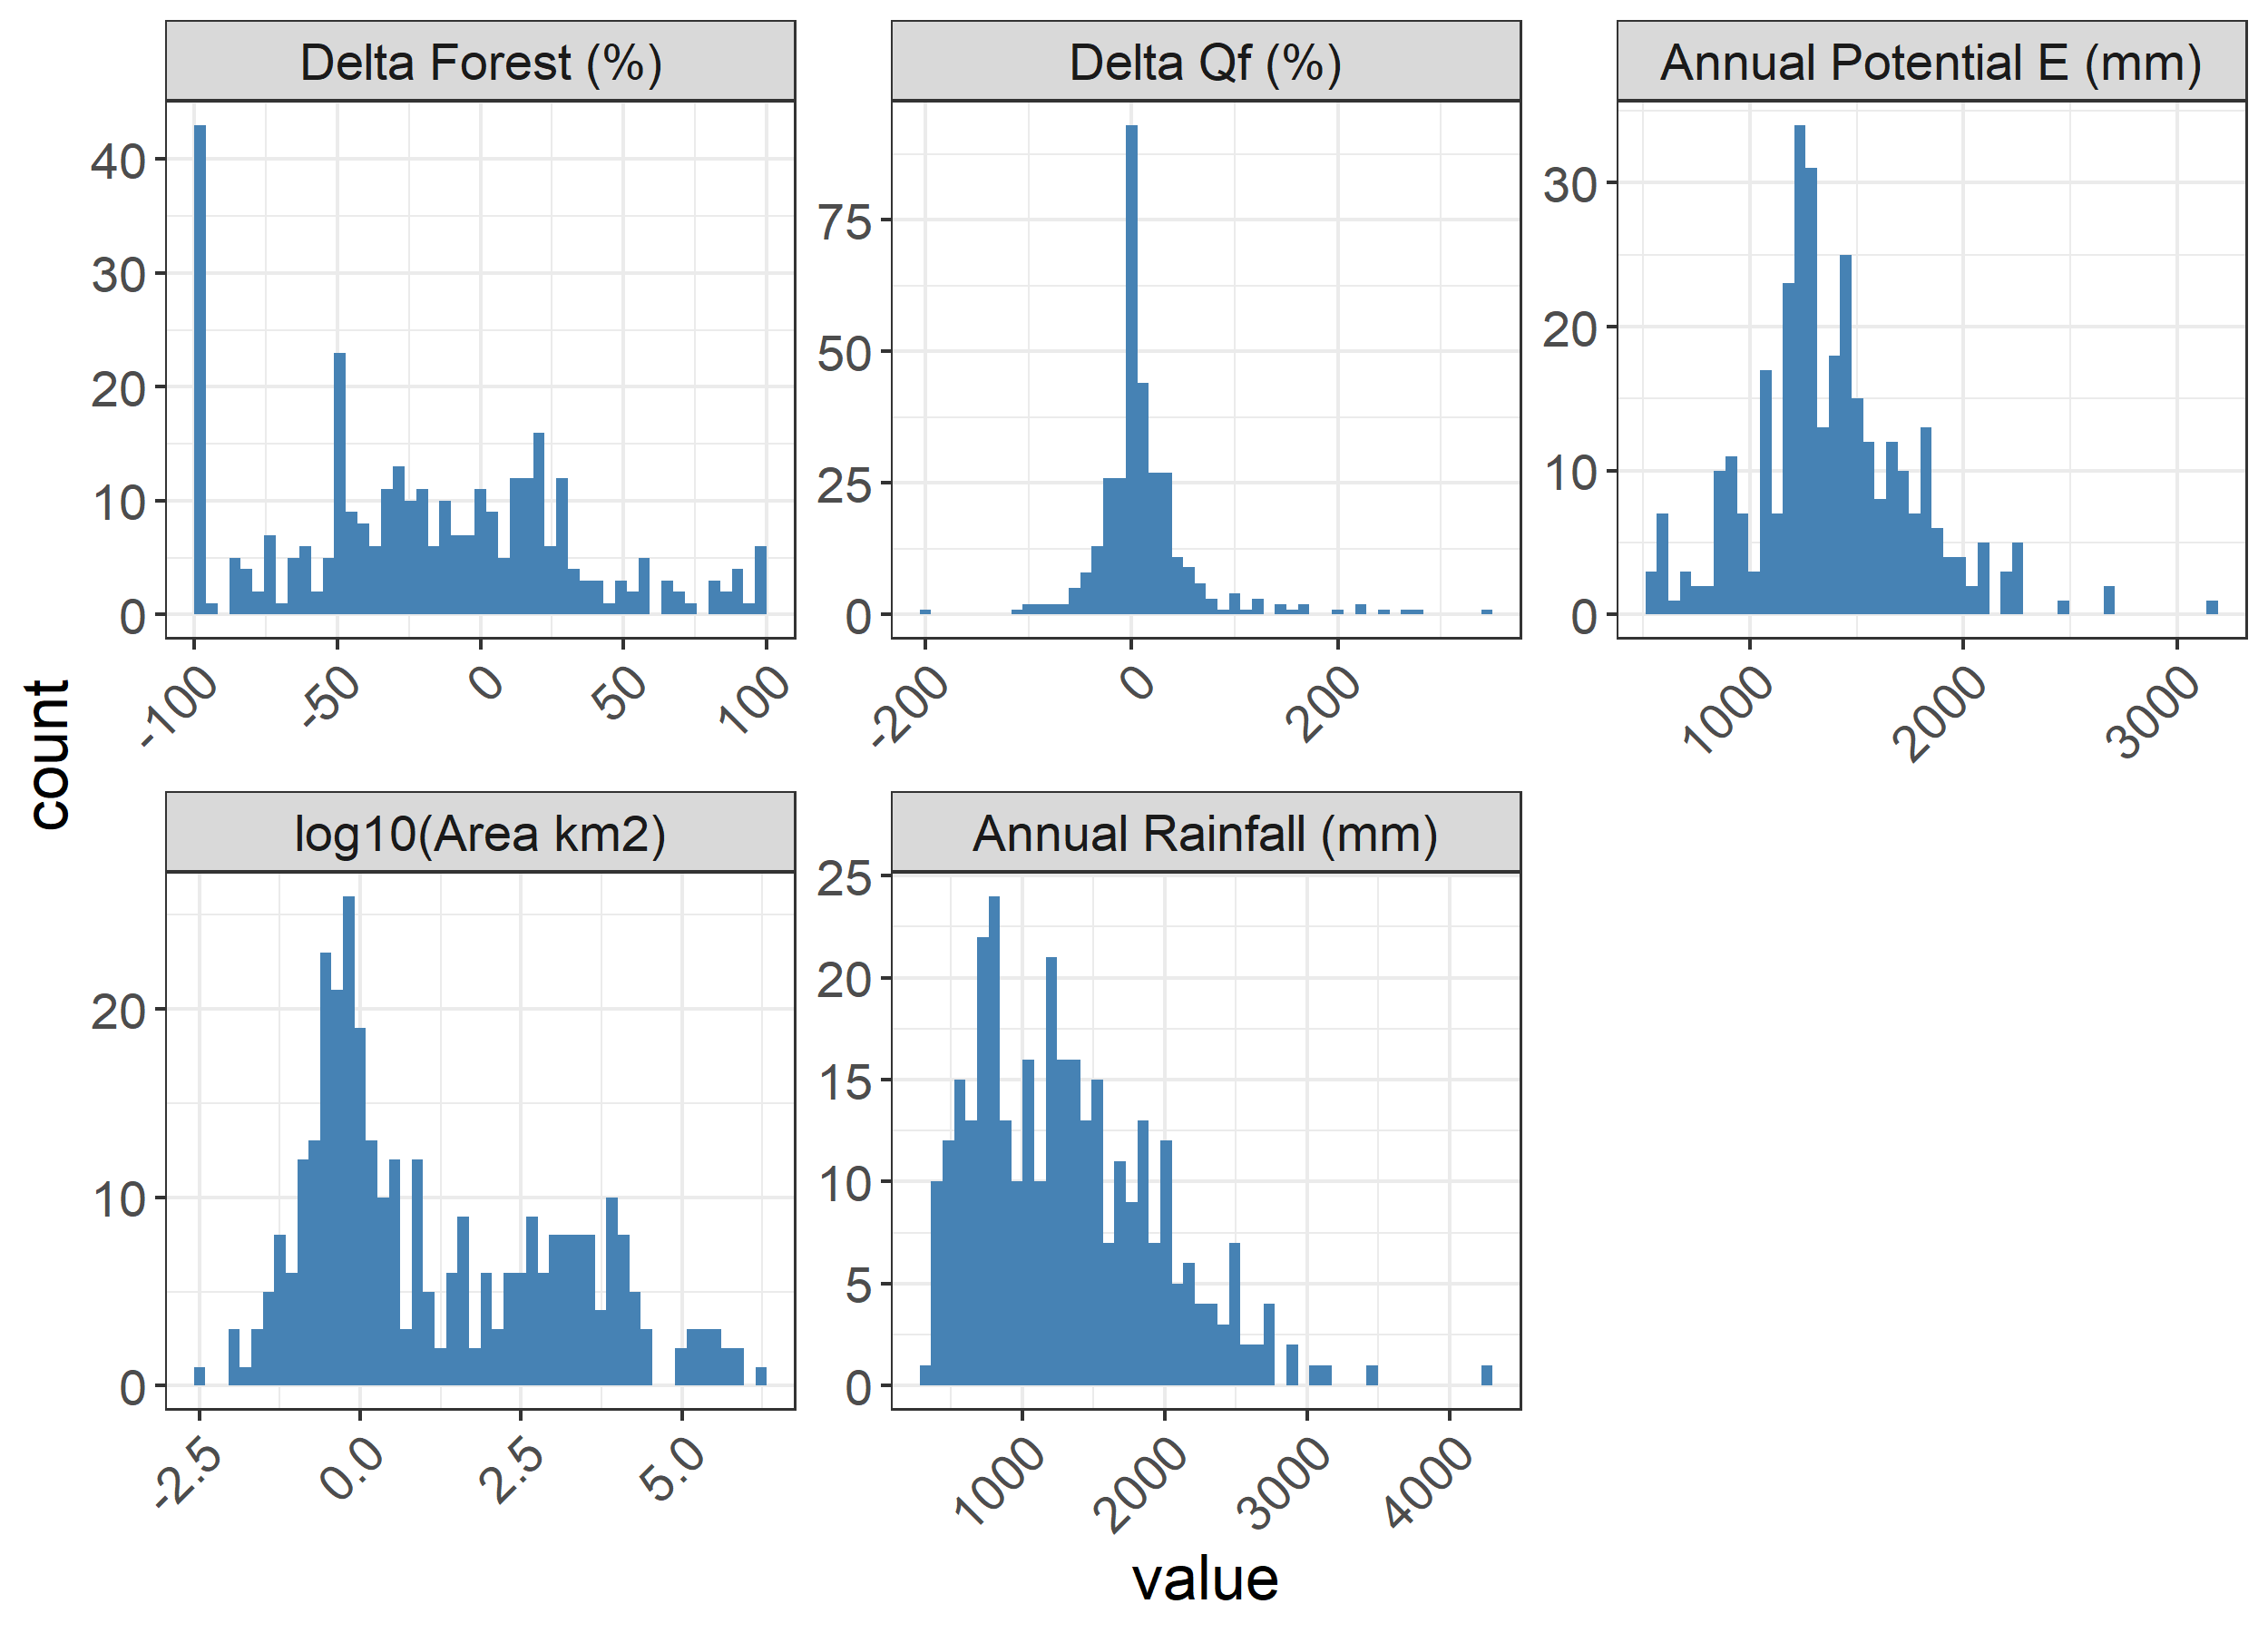
\includegraphics[width=0.9\linewidth]{DataExploration} \caption{Overview of the distributions of some of the variables in the data set}\label{fig:data_graphs}
\end{figure}

\begin{figure}
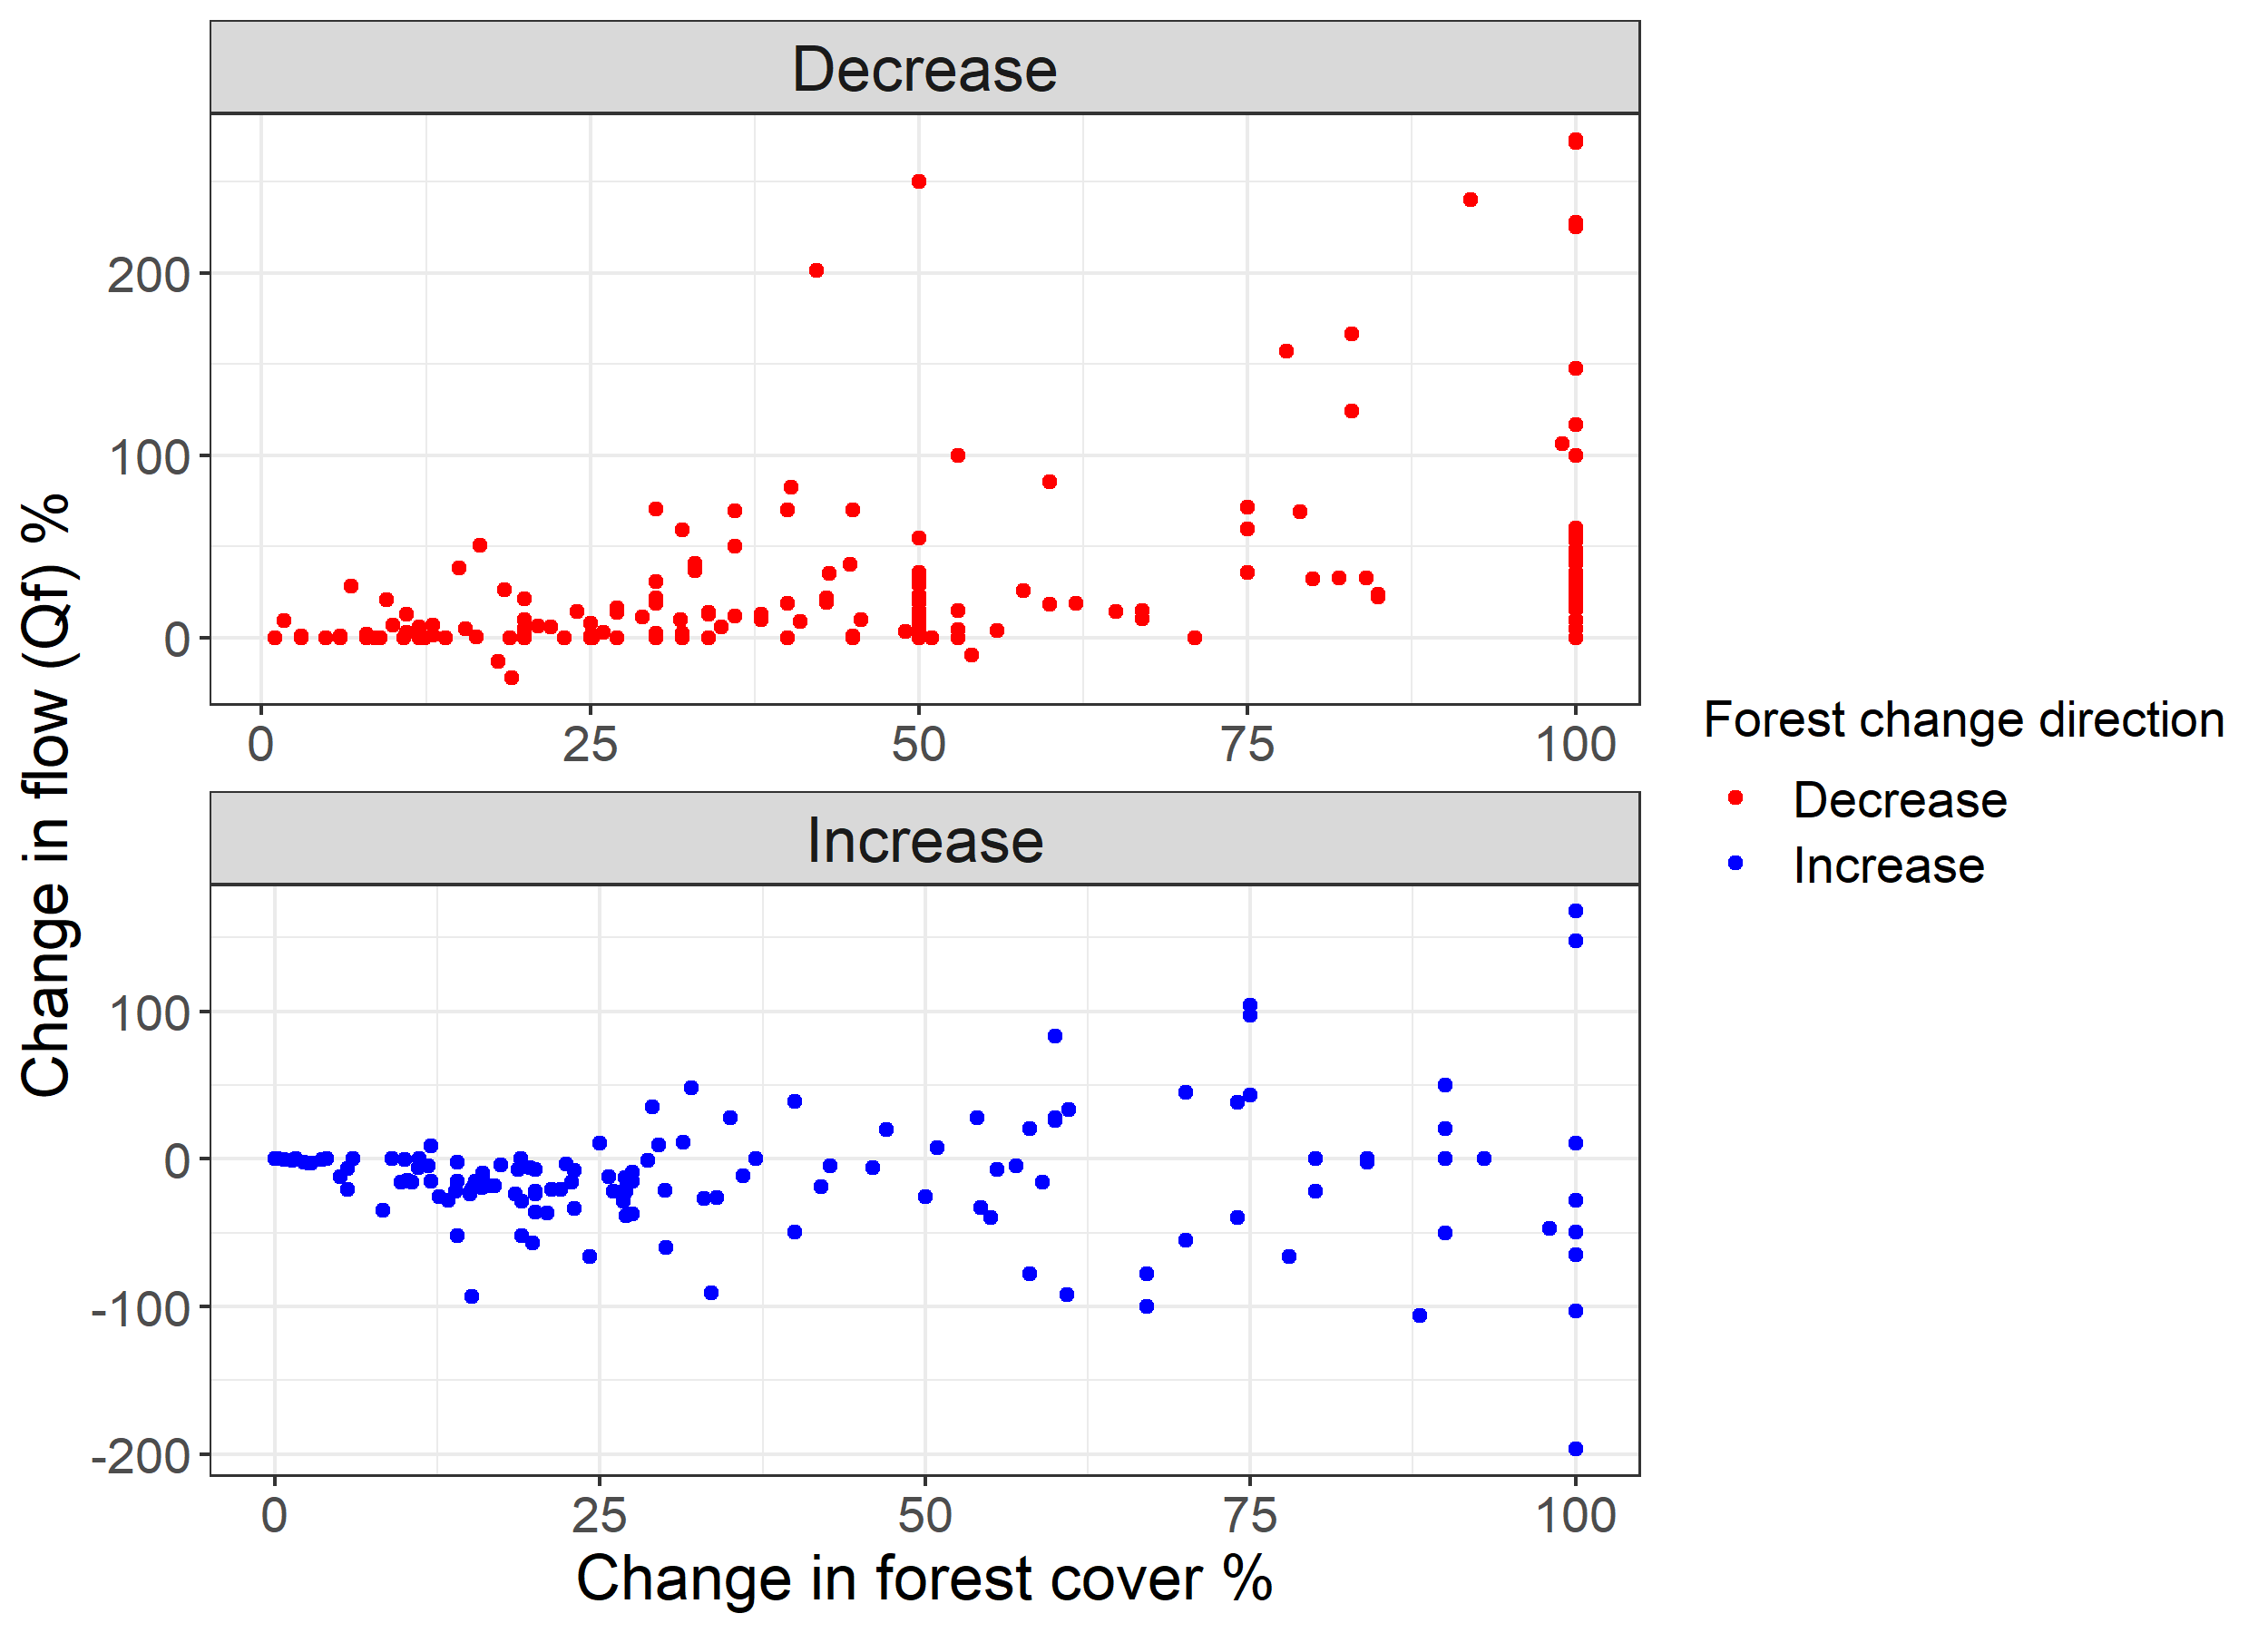
\includegraphics[width=0.9\linewidth]{Increase_decrease} \caption{Changes in flow as a function of increases and decreases in forest cover}\label{fig:increase_decrease}
\end{figure}

This shows that for the data related to forest decreases, there is
almost always a positive flow change. In other words, flow almost always
increased. However, for increases in forest cover, this is not the case,
and flow can both increase and decrease. However in both cases the
variability in the reported change in flow increases with the increase
in forest cover change.

\hypertarget{the-initial-relationship-between-change-in-forest-cover-and-streamflow}{%
\subsection{The initial relationship between change in forest cover and
streamflow}\label{the-initial-relationship-between-change-in-forest-cover-and-streamflow}}

Following Zhang et al. (2017), the first step is to use a linear
regression to investigate the percent change in flow as a result in the
percent change forestry and modulated by the direction of the change,
either an increase in forest cover, or decrease in forest cover:

\[\tag{3}
\begin{aligned}
\Delta \% Q \sim ~ &\Delta \% forest~cover_{positive} + sign_{forest~cover} + \varepsilon
\end{aligned}\]

\begin{longtable}[]{@{}ccccc@{}}
\toprule
\begin{minipage}[b]{0.31\columnwidth}\centering
~\strut
\end{minipage} & \begin{minipage}[b]{0.13\columnwidth}\centering
Estimate\strut
\end{minipage} & \begin{minipage}[b]{0.16\columnwidth}\centering
Std. Error\strut
\end{minipage} & \begin{minipage}[b]{0.12\columnwidth}\centering
t value\strut
\end{minipage} & \begin{minipage}[b]{0.13\columnwidth}\centering
Pr(\textgreater\textbar t\textbar)\strut
\end{minipage}\tabularnewline
\midrule
\endhead
\begin{minipage}[t]{0.31\columnwidth}\centering
\textbf{(Intercept)}\strut
\end{minipage} & \begin{minipage}[t]{0.13\columnwidth}\centering
8.77\strut
\end{minipage} & \begin{minipage}[t]{0.16\columnwidth}\centering
5.52\strut
\end{minipage} & \begin{minipage}[t]{0.12\columnwidth}\centering
1.59\strut
\end{minipage} & \begin{minipage}[t]{0.13\columnwidth}\centering
0.11\strut
\end{minipage}\tabularnewline
\begin{minipage}[t]{0.31\columnwidth}\centering
\textbf{DeltaF\_perc\_pos}\strut
\end{minipage} & \begin{minipage}[t]{0.13\columnwidth}\centering
0.5\strut
\end{minipage} & \begin{minipage}[t]{0.16\columnwidth}\centering
0.09\strut
\end{minipage} & \begin{minipage}[t]{0.12\columnwidth}\centering
5.77\strut
\end{minipage} & \begin{minipage}[t]{0.13\columnwidth}\centering
0\strut
\end{minipage}\tabularnewline
\begin{minipage}[t]{0.31\columnwidth}\centering
\textbf{Forest\_Signincrease}\strut
\end{minipage} & \begin{minipage}[t]{0.13\columnwidth}\centering
-30.9\strut
\end{minipage} & \begin{minipage}[t]{0.16\columnwidth}\centering
5.86\strut
\end{minipage} & \begin{minipage}[t]{0.12\columnwidth}\centering
-5.27\strut
\end{minipage} & \begin{minipage}[t]{0.13\columnwidth}\centering
0\strut
\end{minipage}\tabularnewline
\bottomrule
\end{longtable}

While the overall variance explained in this model is not high with an
adjusted \emph{r\textsuperscript{2}} of 0.19, it clearly supports the
hypothesized relationship between the change in forest cover and the
change in flow. The model suggests that for every 1\% change in forest
cover, on the average, the flow changes 0.5\%. However the change in
flow is different for forest cover decreases compared to forest cover
increases. In fact, forest cover increases decrease flow by 31\% less
than a similar decrease in forest cover causes flow to increase. So
roughly speaking, a 1\% forest cover increase on the average decreases
flow by \((1 - 0.31)*0.5\%\), while a the percentage forest cover
decrease will increase flow by 0.5\%.

It is however it is clear from the lack of explaining power, that there
could be confounding factors, as alluded to in the methods. The obvious
ones being watershed dryness and area (following Zhang et al. (2017)):

\[\tag{4}
\begin{aligned}
\Delta \% Q \sim ~ &\Delta \% forest~cover_{positive} + sign_{forest~cover} + \\ & Pa_{mm} + Area_{km^2} + \varepsilon
\end{aligned}\] Where \(Pa_mm\) is the annual average rainfall in mm.

\begin{longtable}[]{@{}ccccc@{}}
\caption{Summary of the second model, taking into account the annual
rainfall and the area of the watershed}\tabularnewline
\toprule
\begin{minipage}[b]{0.31\columnwidth}\centering
~\strut
\end{minipage} & \begin{minipage}[b]{0.13\columnwidth}\centering
Estimate\strut
\end{minipage} & \begin{minipage}[b]{0.16\columnwidth}\centering
Std. Error\strut
\end{minipage} & \begin{minipage}[b]{0.12\columnwidth}\centering
t value\strut
\end{minipage} & \begin{minipage}[b]{0.13\columnwidth}\centering
Pr(\textgreater\textbar t\textbar)\strut
\end{minipage}\tabularnewline
\midrule
\endfirsthead
\toprule
\begin{minipage}[b]{0.31\columnwidth}\centering
~\strut
\end{minipage} & \begin{minipage}[b]{0.13\columnwidth}\centering
Estimate\strut
\end{minipage} & \begin{minipage}[b]{0.16\columnwidth}\centering
Std. Error\strut
\end{minipage} & \begin{minipage}[b]{0.12\columnwidth}\centering
t value\strut
\end{minipage} & \begin{minipage}[b]{0.13\columnwidth}\centering
Pr(\textgreater\textbar t\textbar)\strut
\end{minipage}\tabularnewline
\midrule
\endhead
\begin{minipage}[t]{0.31\columnwidth}\centering
\textbf{(Intercept)}\strut
\end{minipage} & \begin{minipage}[t]{0.13\columnwidth}\centering
18.94\strut
\end{minipage} & \begin{minipage}[t]{0.16\columnwidth}\centering
7.78\strut
\end{minipage} & \begin{minipage}[t]{0.12\columnwidth}\centering
2.43\strut
\end{minipage} & \begin{minipage}[t]{0.13\columnwidth}\centering
0.02\strut
\end{minipage}\tabularnewline
\begin{minipage}[t]{0.31\columnwidth}\centering
\textbf{DeltaF\_perc\_pos}\strut
\end{minipage} & \begin{minipage}[t]{0.13\columnwidth}\centering
0.5\strut
\end{minipage} & \begin{minipage}[t]{0.16\columnwidth}\centering
0.09\strut
\end{minipage} & \begin{minipage}[t]{0.12\columnwidth}\centering
5.66\strut
\end{minipage} & \begin{minipage}[t]{0.13\columnwidth}\centering
0\strut
\end{minipage}\tabularnewline
\begin{minipage}[t]{0.31\columnwidth}\centering
\textbf{Forest\_Signincrease}\strut
\end{minipage} & \begin{minipage}[t]{0.13\columnwidth}\centering
-31.54\strut
\end{minipage} & \begin{minipage}[t]{0.16\columnwidth}\centering
5.9\strut
\end{minipage} & \begin{minipage}[t]{0.12\columnwidth}\centering
-5.35\strut
\end{minipage} & \begin{minipage}[t]{0.13\columnwidth}\centering
0\strut
\end{minipage}\tabularnewline
\begin{minipage}[t]{0.31\columnwidth}\centering
\textbf{Area\_km2}\strut
\end{minipage} & \begin{minipage}[t]{0.13\columnwidth}\centering
0\strut
\end{minipage} & \begin{minipage}[t]{0.16\columnwidth}\centering
0\strut
\end{minipage} & \begin{minipage}[t]{0.12\columnwidth}\centering
-0.3\strut
\end{minipage} & \begin{minipage}[t]{0.13\columnwidth}\centering
0.77\strut
\end{minipage}\tabularnewline
\begin{minipage}[t]{0.31\columnwidth}\centering
\textbf{Pa\_mm}\strut
\end{minipage} & \begin{minipage}[t]{0.13\columnwidth}\centering
-0.01\strut
\end{minipage} & \begin{minipage}[t]{0.16\columnwidth}\centering
0\strut
\end{minipage} & \begin{minipage}[t]{0.12\columnwidth}\centering
-1.75\strut
\end{minipage} & \begin{minipage}[t]{0.13\columnwidth}\centering
0.08\strut
\end{minipage}\tabularnewline
\bottomrule
\end{longtable}

Including area and annual precipitation does not really improve the
overall explaining power of the model, in fact, annual precipitation
appears to be only a very small confounding factor, representing only a
-0.01/\% partial effect in the change in streamflow, holding all other
factors constant. In contrast to earlier reported studies (Filoso et
al., 2017; Zhang et al., 2017), watershed area has no effect on the
change in stream flow. This supports our approach (in contrast to Zhang
et al. (2017)) to consider watershed area as a continuous variable and
making no separation between larger and smaller watersheds The main
effects remain the change in forest cover and whether this is an
increase or decrease.

\hypertarget{the-effect-of-location-on-the-globe}{%
\subsection{The effect of location on the
globe}\label{the-effect-of-location-on-the-globe}}

\begin{figure}
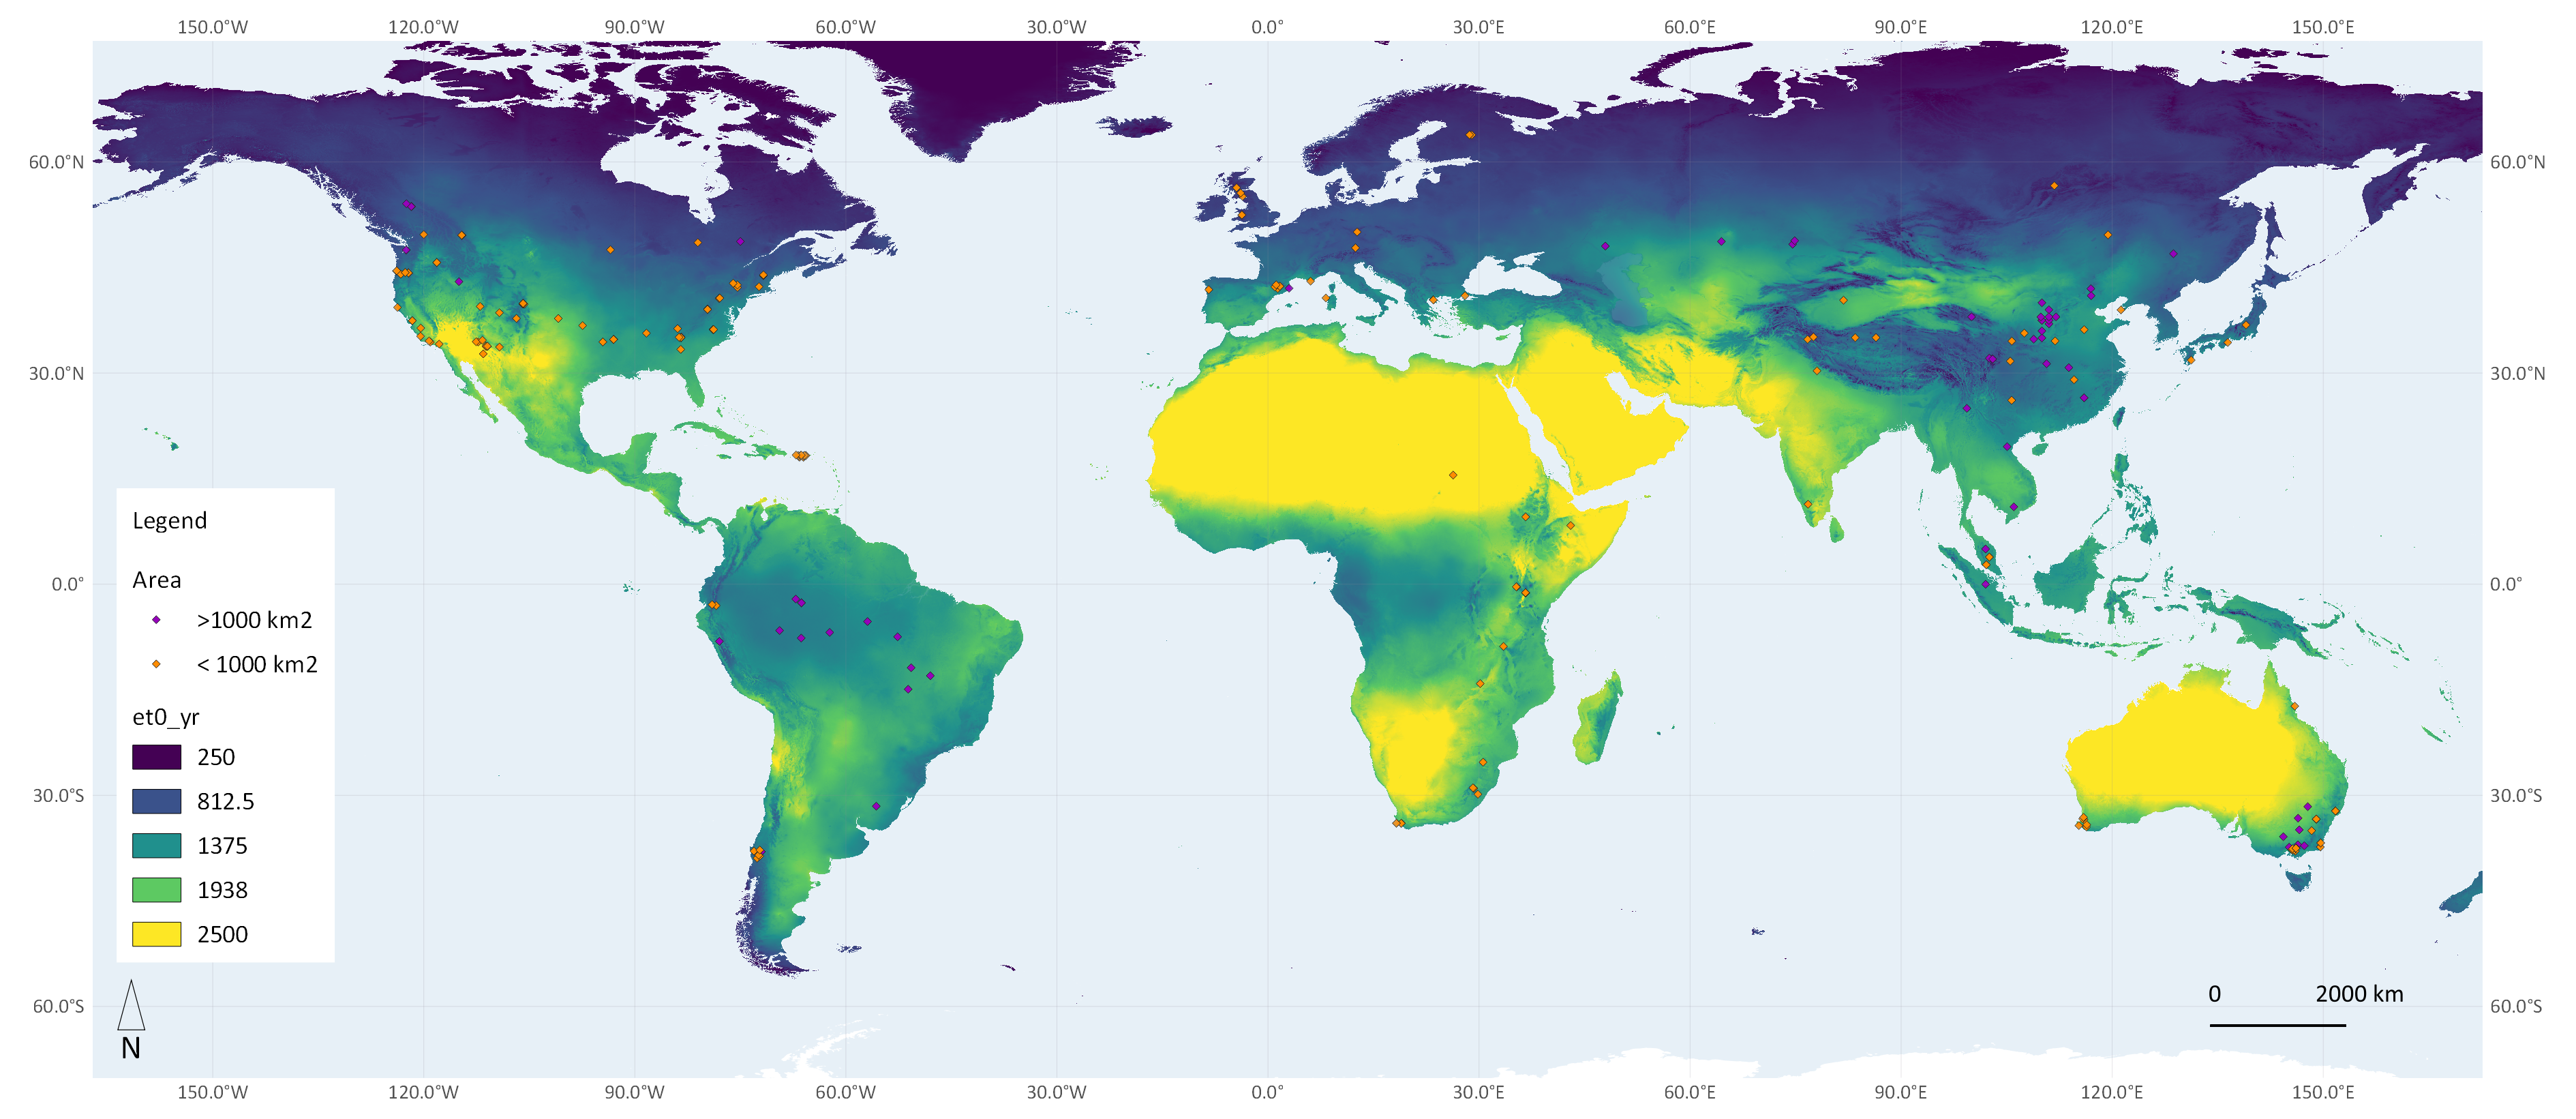
\includegraphics[width=0.9\linewidth]{../../data/FAOET0data2} \caption{Distribution of included watersheds across the globe based on reported or estimated latitude and longitude}\label{fig:global_map}
\end{figure}

As indicated, a further hypothesis relates to whether there is a strong
spatial global gradient as captured by latitude and longitude. As the
global map (@ref(fig:global\_map)) shows, the distribution of case study
watersheds covers multiple continents and shows some distinct clustering
in parts of the world. Of interest is whether the spatial clustering
also indicates a difference in response to forest cover change:

\[\tag{5}
\begin{aligned}
\Delta \% Q \sim ~ &\Delta \% forest~cover_{positive} + sign_{forest~cover} + \\ & Pa_{mm} + Area_{km^2} + Latitude + Longitude + \varepsilon
\end{aligned}\]

\begin{longtable}[]{@{}ccccc@{}}
\caption{Results of the model including Latitude and
Longitude}\tabularnewline
\toprule
\begin{minipage}[b]{0.31\columnwidth}\centering
~\strut
\end{minipage} & \begin{minipage}[b]{0.13\columnwidth}\centering
Estimate\strut
\end{minipage} & \begin{minipage}[b]{0.16\columnwidth}\centering
Std. Error\strut
\end{minipage} & \begin{minipage}[b]{0.12\columnwidth}\centering
t value\strut
\end{minipage} & \begin{minipage}[b]{0.13\columnwidth}\centering
Pr(\textgreater\textbar t\textbar)\strut
\end{minipage}\tabularnewline
\midrule
\endfirsthead
\toprule
\begin{minipage}[b]{0.31\columnwidth}\centering
~\strut
\end{minipage} & \begin{minipage}[b]{0.13\columnwidth}\centering
Estimate\strut
\end{minipage} & \begin{minipage}[b]{0.16\columnwidth}\centering
Std. Error\strut
\end{minipage} & \begin{minipage}[b]{0.12\columnwidth}\centering
t value\strut
\end{minipage} & \begin{minipage}[b]{0.13\columnwidth}\centering
Pr(\textgreater\textbar t\textbar)\strut
\end{minipage}\tabularnewline
\midrule
\endhead
\begin{minipage}[t]{0.31\columnwidth}\centering
\textbf{(Intercept)}\strut
\end{minipage} & \begin{minipage}[t]{0.13\columnwidth}\centering
29.99\strut
\end{minipage} & \begin{minipage}[t]{0.16\columnwidth}\centering
8.65\strut
\end{minipage} & \begin{minipage}[t]{0.12\columnwidth}\centering
3.47\strut
\end{minipage} & \begin{minipage}[t]{0.13\columnwidth}\centering
0\strut
\end{minipage}\tabularnewline
\begin{minipage}[t]{0.31\columnwidth}\centering
\textbf{DeltaF\_perc\_pos}\strut
\end{minipage} & \begin{minipage}[t]{0.13\columnwidth}\centering
0.47\strut
\end{minipage} & \begin{minipage}[t]{0.16\columnwidth}\centering
0.09\strut
\end{minipage} & \begin{minipage}[t]{0.12\columnwidth}\centering
5.4\strut
\end{minipage} & \begin{minipage}[t]{0.13\columnwidth}\centering
0\strut
\end{minipage}\tabularnewline
\begin{minipage}[t]{0.31\columnwidth}\centering
\textbf{Forest\_Signincrease}\strut
\end{minipage} & \begin{minipage}[t]{0.13\columnwidth}\centering
-37.11\strut
\end{minipage} & \begin{minipage}[t]{0.16\columnwidth}\centering
6.09\strut
\end{minipage} & \begin{minipage}[t]{0.12\columnwidth}\centering
-6.09\strut
\end{minipage} & \begin{minipage}[t]{0.13\columnwidth}\centering
0\strut
\end{minipage}\tabularnewline
\begin{minipage}[t]{0.31\columnwidth}\centering
\textbf{Area\_km2}\strut
\end{minipage} & \begin{minipage}[t]{0.13\columnwidth}\centering
0\strut
\end{minipage} & \begin{minipage}[t]{0.16\columnwidth}\centering
0\strut
\end{minipage} & \begin{minipage}[t]{0.12\columnwidth}\centering
-0.59\strut
\end{minipage} & \begin{minipage}[t]{0.13\columnwidth}\centering
0.55\strut
\end{minipage}\tabularnewline
\begin{minipage}[t]{0.31\columnwidth}\centering
\textbf{Pa\_mm}\strut
\end{minipage} & \begin{minipage}[t]{0.13\columnwidth}\centering
-0.01\strut
\end{minipage} & \begin{minipage}[t]{0.16\columnwidth}\centering
0\strut
\end{minipage} & \begin{minipage}[t]{0.12\columnwidth}\centering
-2.17\strut
\end{minipage} & \begin{minipage}[t]{0.13\columnwidth}\centering
0.03\strut
\end{minipage}\tabularnewline
\begin{minipage}[t]{0.31\columnwidth}\centering
\textbf{Latitude}\strut
\end{minipage} & \begin{minipage}[t]{0.13\columnwidth}\centering
-0.29\strut
\end{minipage} & \begin{minipage}[t]{0.16\columnwidth}\centering
0.11\strut
\end{minipage} & \begin{minipage}[t]{0.12\columnwidth}\centering
-2.74\strut
\end{minipage} & \begin{minipage}[t]{0.13\columnwidth}\centering
0.01\strut
\end{minipage}\tabularnewline
\begin{minipage}[t]{0.31\columnwidth}\centering
\textbf{Longitude}\strut
\end{minipage} & \begin{minipage}[t]{0.13\columnwidth}\centering
0.01\strut
\end{minipage} & \begin{minipage}[t]{0.16\columnwidth}\centering
0.03\strut
\end{minipage} & \begin{minipage}[t]{0.12\columnwidth}\centering
0.28\strut
\end{minipage} & \begin{minipage}[t]{0.13\columnwidth}\centering
0.78\strut
\end{minipage}\tabularnewline
\bottomrule
\end{longtable}

This linear model shows that there is a significant gradient in the
Latitude and with annual average rainfall, with watersheds closer to the
equator having lower changes in the runoff compare to watersheds further
away from the equator. This suggests an influence of radiation, which
will be tested next. In addition, the model suggests an influence of the
annual average rainfall, with wetter watersheds having slightly lower
changes in runoff. The total explaining power of the model is still low
with an adjusted \emph{r\textsuperscript{2}} of 0.22 suggesting further
factors that are currently not included in the model.

There is no relationship with Longitude, suggesting that the watersheds
across different continents do not show an East-West direction trend.

\hypertarget{impact-of-the-dryness-index}{%
\subsection{Impact of the dryness
index}\label{impact-of-the-dryness-index}}

Latitude might be indicating an influence of radiation on
evapotranspiration, and most likely related to the dryness index, as
also indicated in Zhang et al. (2017). Increased evapotranspiration
could lead to drier watersheds, unless balanced by rainfall (such as
possibly in the tropics). The North-South trend in dryness would be
related to Latitude. This model introduces the dryness index as a linear
variable and drops the annual average precipitation as a variable, as
dryness is calculated from.

\begin{longtable}[]{@{}ccccc@{}}
\toprule
\begin{minipage}[b]{0.31\columnwidth}\centering
~\strut
\end{minipage} & \begin{minipage}[b]{0.13\columnwidth}\centering
Estimate\strut
\end{minipage} & \begin{minipage}[b]{0.16\columnwidth}\centering
Std. Error\strut
\end{minipage} & \begin{minipage}[b]{0.12\columnwidth}\centering
t value\strut
\end{minipage} & \begin{minipage}[b]{0.13\columnwidth}\centering
Pr(\textgreater\textbar t\textbar)\strut
\end{minipage}\tabularnewline
\midrule
\endhead
\begin{minipage}[t]{0.31\columnwidth}\centering
\textbf{(Intercept)}\strut
\end{minipage} & \begin{minipage}[t]{0.13\columnwidth}\centering
10.27\strut
\end{minipage} & \begin{minipage}[t]{0.16\columnwidth}\centering
7.44\strut
\end{minipage} & \begin{minipage}[t]{0.12\columnwidth}\centering
1.38\strut
\end{minipage} & \begin{minipage}[t]{0.13\columnwidth}\centering
0.17\strut
\end{minipage}\tabularnewline
\begin{minipage}[t]{0.31\columnwidth}\centering
\textbf{DeltaF\_perc\_pos}\strut
\end{minipage} & \begin{minipage}[t]{0.13\columnwidth}\centering
0.46\strut
\end{minipage} & \begin{minipage}[t]{0.16\columnwidth}\centering
0.09\strut
\end{minipage} & \begin{minipage}[t]{0.12\columnwidth}\centering
5.17\strut
\end{minipage} & \begin{minipage}[t]{0.13\columnwidth}\centering
0\strut
\end{minipage}\tabularnewline
\begin{minipage}[t]{0.31\columnwidth}\centering
\textbf{Forest\_Signincrease}\strut
\end{minipage} & \begin{minipage}[t]{0.13\columnwidth}\centering
-37.56\strut
\end{minipage} & \begin{minipage}[t]{0.16\columnwidth}\centering
6.19\strut
\end{minipage} & \begin{minipage}[t]{0.12\columnwidth}\centering
-6.07\strut
\end{minipage} & \begin{minipage}[t]{0.13\columnwidth}\centering
0\strut
\end{minipage}\tabularnewline
\begin{minipage}[t]{0.31\columnwidth}\centering
\textbf{Area\_km2}\strut
\end{minipage} & \begin{minipage}[t]{0.13\columnwidth}\centering
0\strut
\end{minipage} & \begin{minipage}[t]{0.16\columnwidth}\centering
0\strut
\end{minipage} & \begin{minipage}[t]{0.12\columnwidth}\centering
-0.76\strut
\end{minipage} & \begin{minipage}[t]{0.13\columnwidth}\centering
0.45\strut
\end{minipage}\tabularnewline
\begin{minipage}[t]{0.31\columnwidth}\centering
\textbf{Latitude}\strut
\end{minipage} & \begin{minipage}[t]{0.13\columnwidth}\centering
-0.28\strut
\end{minipage} & \begin{minipage}[t]{0.16\columnwidth}\centering
0.11\strut
\end{minipage} & \begin{minipage}[t]{0.12\columnwidth}\centering
-2.66\strut
\end{minipage} & \begin{minipage}[t]{0.13\columnwidth}\centering
0.01\strut
\end{minipage}\tabularnewline
\begin{minipage}[t]{0.31\columnwidth}\centering
\textbf{Longitude}\strut
\end{minipage} & \begin{minipage}[t]{0.13\columnwidth}\centering
0.01\strut
\end{minipage} & \begin{minipage}[t]{0.16\columnwidth}\centering
0.03\strut
\end{minipage} & \begin{minipage}[t]{0.12\columnwidth}\centering
0.4\strut
\end{minipage} & \begin{minipage}[t]{0.13\columnwidth}\centering
0.69\strut
\end{minipage}\tabularnewline
\begin{minipage}[t]{0.31\columnwidth}\centering
\textbf{Dryness}\strut
\end{minipage} & \begin{minipage}[t]{0.13\columnwidth}\centering
6.1\strut
\end{minipage} & \begin{minipage}[t]{0.16\columnwidth}\centering
3.09\strut
\end{minipage} & \begin{minipage}[t]{0.12\columnwidth}\centering
1.97\strut
\end{minipage} & \begin{minipage}[t]{0.13\columnwidth}\centering
0.05\strut
\end{minipage}\tabularnewline
\bottomrule
\end{longtable}

The results from this model confirm that dryness is a significant
confounding factor of the change in streamflow as function of the change
in forest cover change. In fact if the dryness index doubles
(remembering that Dryness = 1 when E0 = Pa, so in this case E0 = 2*Pa,
which is very dry), the change in runoff is \textasciitilde14\% greater.
However, more interesting, Latitude remains a significant predictor with
each degree in latitude causing an -0.31\% change in runoff. This
indicates that Dryness (i.e.~an increase in radiation) alone does not
explain the trend in the Latitude and some other unknown confounding
factor is captured by Latitude.

However, the result also indicates possible issues with the data, some
of the Dryness values are very large (\textgreater{} 4) and these values
have high leverage in the data. These watersheds are listed in Table XX:

\begin{longtable}[]{@{}ccc@{}}
\toprule
\begin{minipage}[b]{0.14\columnwidth}\centering
Latitude\strut
\end{minipage} & \begin{minipage}[b]{0.15\columnwidth}\centering
Longitude\strut
\end{minipage} & \begin{minipage}[b]{0.42\columnwidth}\centering
Watershed name\strut
\end{minipage}\tabularnewline
\midrule
\endhead
\begin{minipage}[t]{0.14\columnwidth}\centering
34.67\strut
\end{minipage} & \begin{minipage}[t]{0.15\columnwidth}\centering
-111.7\strut
\end{minipage} & \begin{minipage}[t]{0.42\columnwidth}\centering
Beaver Creek, AZ \#3-2\strut
\end{minipage}\tabularnewline
\begin{minipage}[t]{0.14\columnwidth}\centering
36.4\strut
\end{minipage} & \begin{minipage}[t]{0.15\columnwidth}\centering
-120.4\strut
\end{minipage} & \begin{minipage}[t]{0.42\columnwidth}\centering
Cantua\strut
\end{minipage}\tabularnewline
\begin{minipage}[t]{0.14\columnwidth}\centering
34.43\strut
\end{minipage} & \begin{minipage}[t]{0.15\columnwidth}\centering
-112.3\strut
\end{minipage} & \begin{minipage}[t]{0.42\columnwidth}\centering
White Spar, Ariz., U.S.A, B\strut
\end{minipage}\tabularnewline
\begin{minipage}[t]{0.14\columnwidth}\centering
32.74\strut
\end{minipage} & \begin{minipage}[t]{0.15\columnwidth}\centering
-111.5\strut
\end{minipage} & \begin{minipage}[t]{0.42\columnwidth}\centering
Natural DRDages, Ariz., U.S.A, A\strut
\end{minipage}\tabularnewline
\bottomrule
\end{longtable}

\begin{verbatim}
## 
## Family: gaussian 
## Link function: identity 
## 
## Formula:
## DeltaQf_perc ~ DeltaF_perc_pos + Forest_Sign + s(Area_km2, bs = "ts") + 
##     s(Dryness, bs = "ts") + s(length, bs = "ts") + Latitude
## 
## Parametric coefficients:
##                      Estimate Std. Error t value Pr(>|t|)    
## (Intercept)          18.85584    5.84673   3.225 0.001419 ** 
## DeltaF_perc_pos       0.37334    0.09042   4.129 4.90e-05 ***
## Forest_Signincrease -33.25371    6.40370  -5.193 4.15e-07 ***
## Latitude             -0.29544    0.08775  -3.367 0.000873 ***
## ---
## Signif. codes:  0 '***' 0.001 '**' 0.01 '*' 0.05 '.' 0.1 ' ' 1
## 
## Approximate significance of smooth terms:
##                   edf Ref.df     F p-value  
## s(Area_km2) 3.174e-06      9 0.000  0.3914  
## s(Dryness)  1.293e-05      9 0.000  0.5926  
## s(length)   5.991e+00      9 1.221  0.0779 .
## ---
## Signif. codes:  0 '***' 0.001 '**' 0.01 '*' 0.05 '.' 0.1 ' ' 1
## 
## R-sq.(adj) =  0.227   Deviance explained = 25.2%
## GCV =   2018  Scale est. = 1944.1    n = 273
\end{verbatim}

\begin{verbatim}
## 
## Family: gaussian 
## Link function: identity 
## 
## Formula:
## DeltaQf_perc ~ DeltaF_perc_pos + Forest_Sign + s(Area_km2, bs = "ts") + 
##     s(Dryness, bs = "ts") + s(Latitude, bs = "ts") + s(length, 
##     bs = "ts") + Precip_data_type + Assessment_technique + Forest_type + 
##     Hydrological_regime
## 
## Parametric coefficients:
##                             Estimate Std. Error t value Pr(>|t|)    
## (Intercept)                   2.5565    25.5148   0.100 0.920272    
## DeltaF_perc_pos               0.3234     0.1058   3.057 0.002482 ** 
## Forest_Signincrease         -27.2070     7.5951  -3.582 0.000411 ***
## Precip_data_typeOB            2.9296    15.9005   0.184 0.853974    
## Precip_data_typeSG           23.9270    18.5848   1.287 0.199159    
## Assessment_techniqueEA, HM   14.8215    46.1143   0.321 0.748176    
## Assessment_techniqueHM       -7.5091    18.4252  -0.408 0.683967    
## Assessment_techniquePWE       8.9562    19.7884   0.453 0.651240    
## Assessment_techniquePWE, HM  19.6741    52.6286   0.374 0.708856    
## Assessment_techniqueQPW      -7.3110    28.3315  -0.258 0.796583    
## Assessment_techniqueSH        2.8647    18.4698   0.155 0.876871    
## Forest_typeCF                 4.9185     9.2133   0.534 0.593935    
## Forest_typeMF               -10.6875     9.6354  -1.109 0.268444    
## Hydrological_regimeSD         6.9324    10.5522   0.657 0.511825    
## ---
## Signif. codes:  0 '***' 0.001 '**' 0.01 '*' 0.05 '.' 0.1 ' ' 1
## 
## Approximate significance of smooth terms:
##                   edf Ref.df     F p-value   
## s(Area_km2) 1.754e-07      9 0.000 0.50299   
## s(Dryness)  1.784e-06      9 0.000 0.87130   
## s(Latitude) 3.607e+00      9 1.648 0.00213 **
## s(length)   5.815e+00      9 1.067 0.11589   
## ---
## Signif. codes:  0 '***' 0.001 '**' 0.01 '*' 0.05 '.' 0.1 ' ' 1
## 
## R-sq.(adj) =  0.231   Deviance explained = 29.6%
## GCV = 2158.9  Scale est. = 1969.5    n = 267
\end{verbatim}

\begin{Shaded}
\begin{Highlighting}[]
\NormalTok{model6_reduc <-}\StringTok{ }\KeywordTok{gam}\NormalTok{(DeltaQf_perc }\OperatorTok{~}\StringTok{ }\NormalTok{DeltaF_perc_pos }\OperatorTok{+}\StringTok{ }\NormalTok{Forest_Sign }\OperatorTok{+}\StringTok{ }
\StringTok{                    }\KeywordTok{s}\NormalTok{(Dryness, }\DataTypeTok{bs=}\StringTok{"ts"}\NormalTok{ ) }\OperatorTok{+}\StringTok{ }\KeywordTok{s}\NormalTok{(Latitude, }\DataTypeTok{bs=}\StringTok{"ts"}\NormalTok{) }\OperatorTok{+}\StringTok{ }
\StringTok{                      }\KeywordTok{s}\NormalTok{(Area_km2, }\DataTypeTok{bs=}\StringTok{"ts"}\NormalTok{) }\OperatorTok{+}\StringTok{  }\KeywordTok{s}\NormalTok{(length, }\DataTypeTok{bs=}\StringTok{"ts"}\NormalTok{) }\OperatorTok{+}
\StringTok{                    }\NormalTok{Assessment_technique }\OperatorTok{+}
\StringTok{                    }\NormalTok{Hydrological_regime, }\DataTypeTok{data =}\NormalTok{ Zhang_all2)}
\KeywordTok{summary}\NormalTok{(model6_reduc)}
\end{Highlighting}
\end{Shaded}

\begin{verbatim}
## 
## Family: gaussian 
## Link function: identity 
## 
## Formula:
## DeltaQf_perc ~ DeltaF_perc_pos + Forest_Sign + s(Dryness, bs = "ts") + 
##     s(Latitude, bs = "ts") + s(Area_km2, bs = "ts") + s(length, 
##     bs = "ts") + Assessment_technique + Hydrological_regime
## 
## Parametric coefficients:
##                             Estimate Std. Error t value Pr(>|t|)    
## (Intercept)                  11.5706    17.3998   0.665  0.50666    
## DeltaF_perc_pos               0.3094     0.1038   2.979  0.00317 ** 
## Forest_Signincrease         -29.9159     7.1426  -4.188 3.88e-05 ***
## Assessment_techniqueEA, HM   11.4108    45.6037   0.250  0.80262    
## Assessment_techniqueHM       -4.6254    17.2047  -0.269  0.78827    
## Assessment_techniquePWE       3.8045    18.5150   0.205  0.83736    
## Assessment_techniquePWE, HM  17.3096    50.9143   0.340  0.73416    
## Assessment_techniqueQPW     -14.1255    26.9676  -0.524  0.60088    
## Assessment_techniqueSH       -0.6693    17.6262  -0.038  0.96974    
## Hydrological_regimeSD        12.3022     8.4529   1.455  0.14680    
## ---
## Signif. codes:  0 '***' 0.001 '**' 0.01 '*' 0.05 '.' 0.1 ' ' 1
## 
## Approximate significance of smooth terms:
##                   edf Ref.df     F  p-value    
## s(Dryness)  1.026e-05      9 0.000 0.885487    
## s(Latitude) 3.300e+00      9 1.829 0.000683 ***
## s(Area_km2) 2.280e-06      9 0.000 0.848293    
## s(length)   5.575e+00      9 0.901 0.176727    
## ---
## Signif. codes:  0 '***' 0.001 '**' 0.01 '*' 0.05 '.' 0.1 ' ' 1
## 
## R-sq.(adj) =  0.228   Deviance explained = 27.9%
## GCV = 2085.2  Scale est. = 1941.1    n = 273
\end{verbatim}

Clearly Latitude is masking other factors including the assessment
technique and the forest type

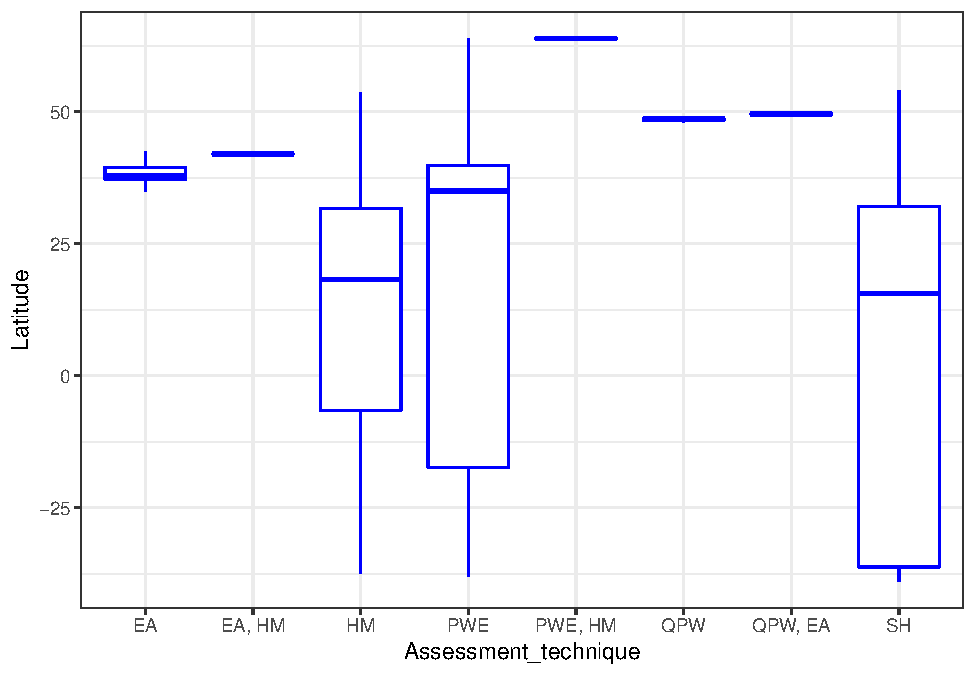
\includegraphics{Forest_and_Water_files/figure-latex/unnamed-chunk-18-1.pdf}

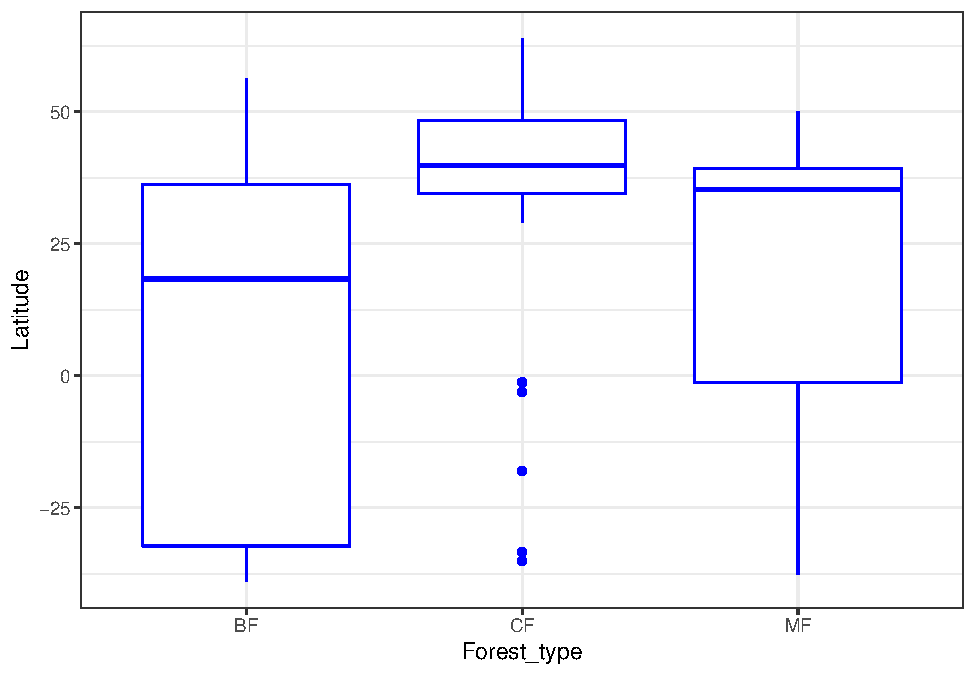
\includegraphics{Forest_and_Water_files/figure-latex/unnamed-chunk-19-1.pdf}

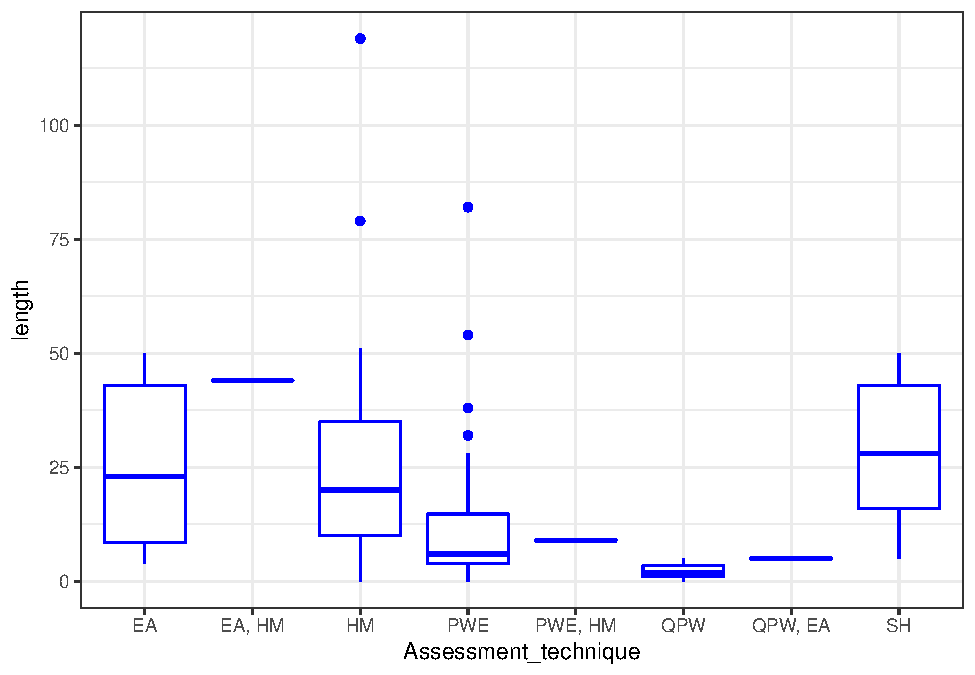
\includegraphics{Forest_and_Water_files/figure-latex/unnamed-chunk-20-1.pdf}

Clearly all have at least some relationship with Latitude, therefore are
being masked if Latitude is included in the model.

\begin{Shaded}
\begin{Highlighting}[]
\NormalTok{model7_noLat <-}\StringTok{ }\KeywordTok{gam}\NormalTok{(DeltaQf_perc }\OperatorTok{~}\StringTok{ }\NormalTok{DeltaF_perc_pos }\OperatorTok{+}\StringTok{ }\NormalTok{Forest_Sign }\OperatorTok{+}\StringTok{ }
\StringTok{                    }\KeywordTok{s}\NormalTok{(Dryness, }\DataTypeTok{bs=}\StringTok{"ts"}\NormalTok{ ) }\OperatorTok{+}\StringTok{ }
\StringTok{                      }\KeywordTok{s}\NormalTok{(Area_km2, }\DataTypeTok{bs=}\StringTok{"ts"}\NormalTok{)  }\OperatorTok{+}
\StringTok{                    }\NormalTok{Precip_data_type }\OperatorTok{+}\StringTok{  }\NormalTok{Assessment_technique }\OperatorTok{+}\StringTok{ }\NormalTok{Forest_type }\OperatorTok{+}
\StringTok{                    }\NormalTok{Hydrological_regime, }\DataTypeTok{data =}\NormalTok{ Zhang_all2)}
\KeywordTok{summary}\NormalTok{(model7_noLat)}
\end{Highlighting}
\end{Shaded}

\begin{verbatim}
## 
## Family: gaussian 
## Link function: identity 
## 
## Formula:
## DeltaQf_perc ~ DeltaF_perc_pos + Forest_Sign + s(Dryness, bs = "ts") + 
##     s(Area_km2, bs = "ts") + Precip_data_type + Assessment_technique + 
##     Forest_type + Hydrological_regime
## 
## Parametric coefficients:
##                             Estimate Std. Error t value Pr(>|t|)    
## (Intercept)                 -12.5291    22.7513  -0.551 0.582282    
## DeltaF_perc_pos               0.4348     0.1033   4.209 3.46e-05 ***
## Forest_Signincrease         -27.2295     7.6821  -3.545 0.000461 ***
## Precip_data_typeOB          -12.4249    15.4195  -0.806 0.421049    
## Precip_data_typeSG           11.5676    17.1018   0.676 0.499348    
## Assessment_techniqueEA, HM   19.1901    50.7190   0.378 0.705450    
## Assessment_techniqueHM       21.6621    17.2625   1.255 0.210578    
## Assessment_techniquePWE      42.2758    17.2104   2.456 0.014642 *  
## Assessment_techniquePWE, HM  23.5495    52.6315   0.447 0.654903    
## Assessment_techniqueQPW      22.1990    27.1887   0.816 0.414924    
## Assessment_techniqueQPW, EA  41.0844    30.1936   1.361 0.174707    
## Assessment_techniqueSH       38.3711    18.7848   2.043 0.042025 *  
## Forest_typeCF                -3.7900     9.7088  -0.390 0.696562    
## Forest_typeMF               -16.3363     9.3408  -1.749 0.081404 .  
## Hydrological_regimeSD        -1.1868    10.9105  -0.109 0.913460    
## ---
## Signif. codes:  0 '***' 0.001 '**' 0.01 '*' 0.05 '.' 0.1 ' ' 1
## 
## Approximate significance of smooth terms:
##                   edf Ref.df     F p-value  
## s(Dryness)  3.995e+00      9 1.162   0.024 *
## s(Area_km2) 2.228e-07      9 0.000   0.439  
## ---
## Signif. codes:  0 '***' 0.001 '**' 0.01 '*' 0.05 '.' 0.1 ' ' 1
## 
## R-sq.(adj) =  0.202   Deviance explained =   25%
## GCV =   2510  Scale est. = 2350      n = 298
\end{verbatim}

\begin{Shaded}
\begin{Highlighting}[]
\KeywordTok{plot}\NormalTok{(model7_noLat)}
\end{Highlighting}
\end{Shaded}

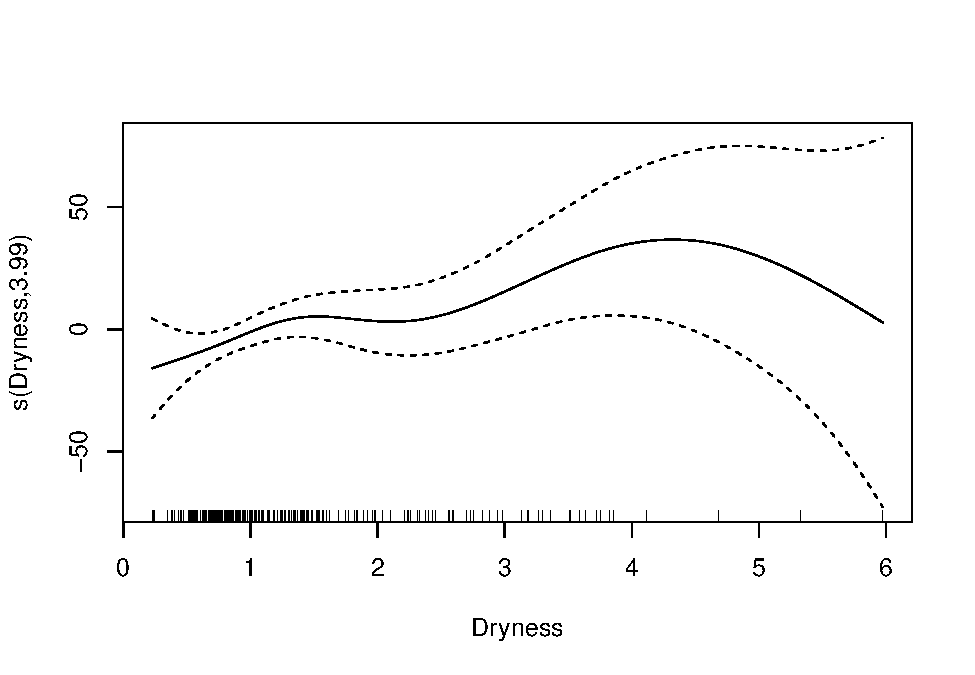
\includegraphics{Forest_and_Water_files/figure-latex/model7_noLat-1.pdf}
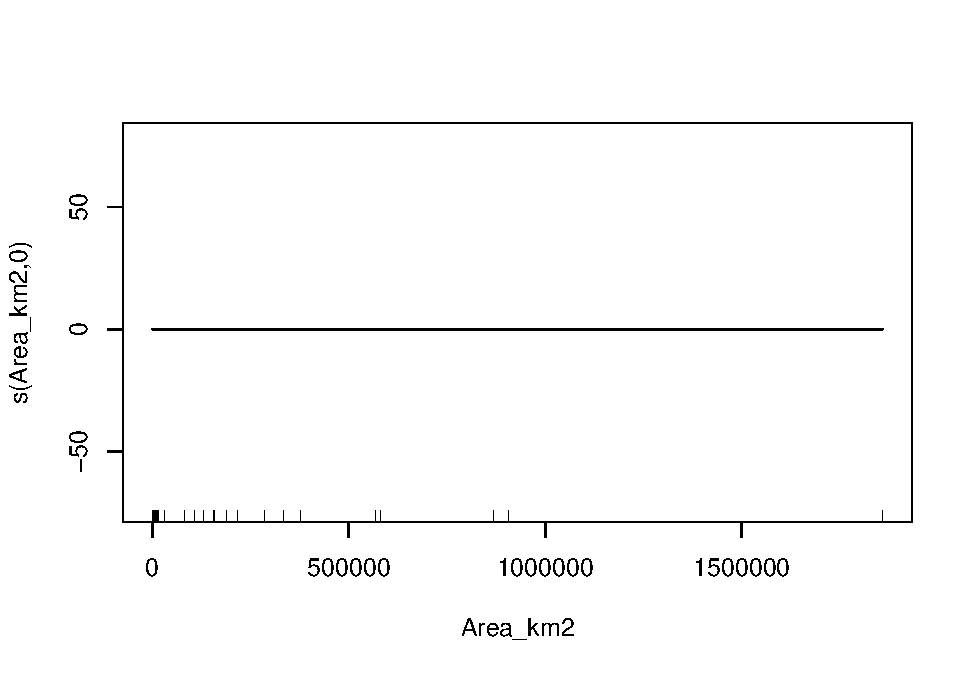
\includegraphics{Forest_and_Water_files/figure-latex/model7_noLat-2.pdf}

\begin{verbatim}
## Warning: Removed 32 rows containing missing values (geom_point).
\end{verbatim}

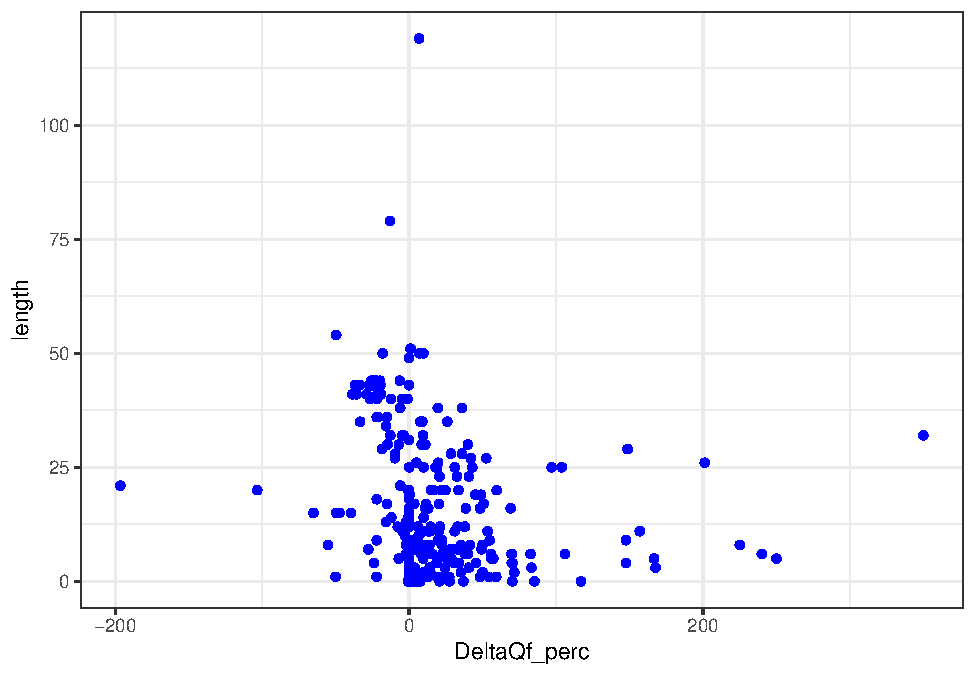
\includegraphics{Forest_and_Water_files/figure-latex/unnamed-chunk-21-1.pdf}

In drier watersheds, changes in forest cover have greater impact on
flow, which is similar to Zhang et al. (2017). This is most likely
because in these watersheds the overall flow is surface flow dominated
and therefore the buffering that is afforded by the groundwater inputs
is not as great. As we don't have a separate variable for groundwater
inputs (although this effect is estimated in many studies), we cannot
analyse this effect separately.

In contrast to Filoso et al. (2017), we also did not identify an effect
of the

Given how skewed Dryness is due tot he few watersheds that have very
high dryness values, it is worth investigating what excluding these 4
watersheds from the data means for the relationships.

\begin{Shaded}
\begin{Highlighting}[]
\NormalTok{model7_noLatb <-}\StringTok{ }\KeywordTok{gam}\NormalTok{(DeltaQf_perc }\OperatorTok{~}\StringTok{ }\NormalTok{DeltaF_perc_pos }\OperatorTok{+}\StringTok{ }\NormalTok{Forest_Sign }\OperatorTok{+}\StringTok{ }
\StringTok{                    }\KeywordTok{s}\NormalTok{(Dryness, }\DataTypeTok{bs=}\StringTok{"ts"}\NormalTok{ ) }\OperatorTok{+}\StringTok{ }\CommentTok{#s(Latitude, bs="ts") + }
\StringTok{                      }\KeywordTok{s}\NormalTok{(Area_km2, }\DataTypeTok{bs=}\StringTok{"ts"}\NormalTok{) }\OperatorTok{+}
\StringTok{                    }\NormalTok{Precip_data_type }\OperatorTok{+}\StringTok{  }\NormalTok{Assessment_technique }\OperatorTok{+}\StringTok{ }\NormalTok{Forest_type }\OperatorTok{+}
\StringTok{                    }\NormalTok{Hydrological_regime, }\DataTypeTok{data =}\NormalTok{ Zhang_all2 }\OperatorTok\StringTok{ }\KeywordTok{filter}\NormalTok{(Dryness }\OperatorTok{<}\StringTok{ }\DecValTok{4}\NormalTok{))}
\KeywordTok{summary}\NormalTok{(model7_noLatb)}
\end{Highlighting}
\end{Shaded}

\begin{verbatim}
## 
## Family: gaussian 
## Link function: identity 
## 
## Formula:
## DeltaQf_perc ~ DeltaF_perc_pos + Forest_Sign + s(Dryness, bs = "ts") + 
##     s(Area_km2, bs = "ts") + Precip_data_type + Assessment_technique + 
##     Forest_type + Hydrological_regime
## 
## Parametric coefficients:
##                             Estimate Std. Error t value Pr(>|t|)    
## (Intercept)                 -16.8716    22.8324  -0.739 0.460577    
## DeltaF_perc_pos               0.4205     0.1036   4.060 6.41e-05 ***
## Forest_Signincrease         -27.4323     7.6284  -3.596 0.000383 ***
## Precip_data_typeOB          -12.8820    15.2846  -0.843 0.400065    
## Precip_data_typeSG           11.9340    16.9606   0.704 0.482257    
## Assessment_techniqueEA, HM   25.8163    50.4996   0.511 0.609607    
## Assessment_techniqueHM       26.4681    17.4660   1.515 0.130815    
## Assessment_techniquePWE      48.3282    17.6030   2.745 0.006440 ** 
## Assessment_techniquePWE, HM  29.5466    52.3323   0.565 0.572808    
## Assessment_techniqueQPW      29.1804    27.2233   1.072 0.284707    
## Assessment_techniqueQPW, EA  48.6163    30.1921   1.610 0.108492    
## Assessment_techniqueSH       43.7353    18.9899   2.303 0.022019 *  
## Forest_typeCF                -4.2723     9.6304  -0.444 0.657661    
## Forest_typeMF               -14.2554     9.4382  -1.510 0.132089    
## Hydrological_regimeSD        -2.6825    10.8541  -0.247 0.804980    
## ---
## Signif. codes:  0 '***' 0.001 '**' 0.01 '*' 0.05 '.' 0.1 ' ' 1
## 
## Approximate significance of smooth terms:
##                   edf Ref.df     F p-value   
## s(Dryness)  3.374e+00      9 1.576 0.00703 **
## s(Area_km2) 3.036e-09      9 0.000 0.41938   
## ---
## Signif. codes:  0 '***' 0.001 '**' 0.01 '*' 0.05 '.' 0.1 ' ' 1
## 
## R-sq.(adj) =  0.209   Deviance explained = 25.6%
## GCV = 2462.7  Scale est. = 2308.7    n = 294
\end{verbatim}

\begin{Shaded}
\begin{Highlighting}[]
\KeywordTok{plot}\NormalTok{(model7_noLatb)}
\end{Highlighting}
\end{Shaded}

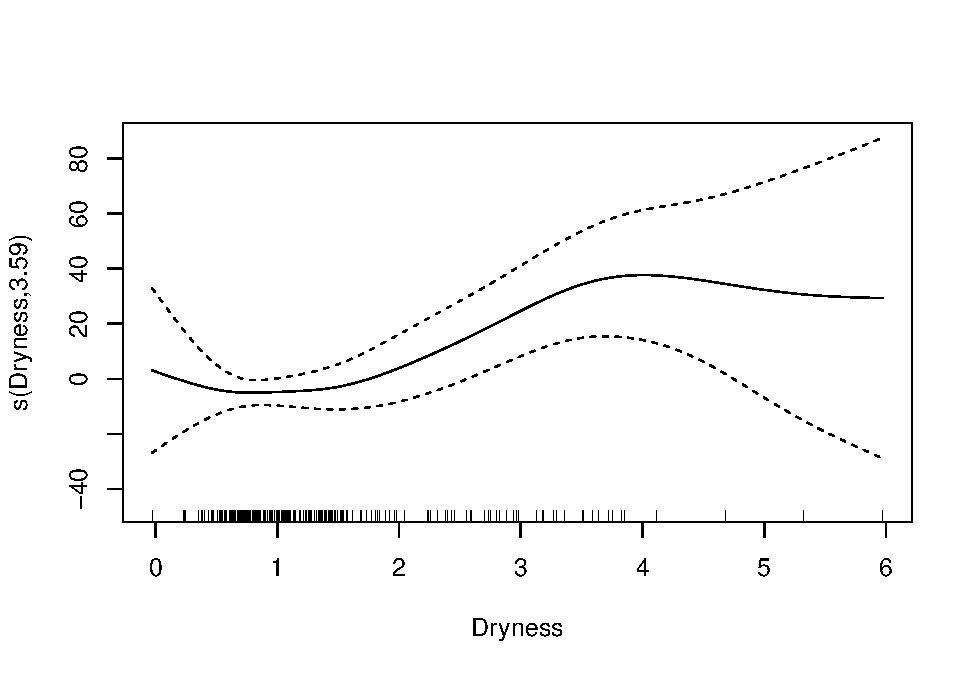
\includegraphics{Forest_and_Water_files/figure-latex/model7_noLatb-1.pdf}
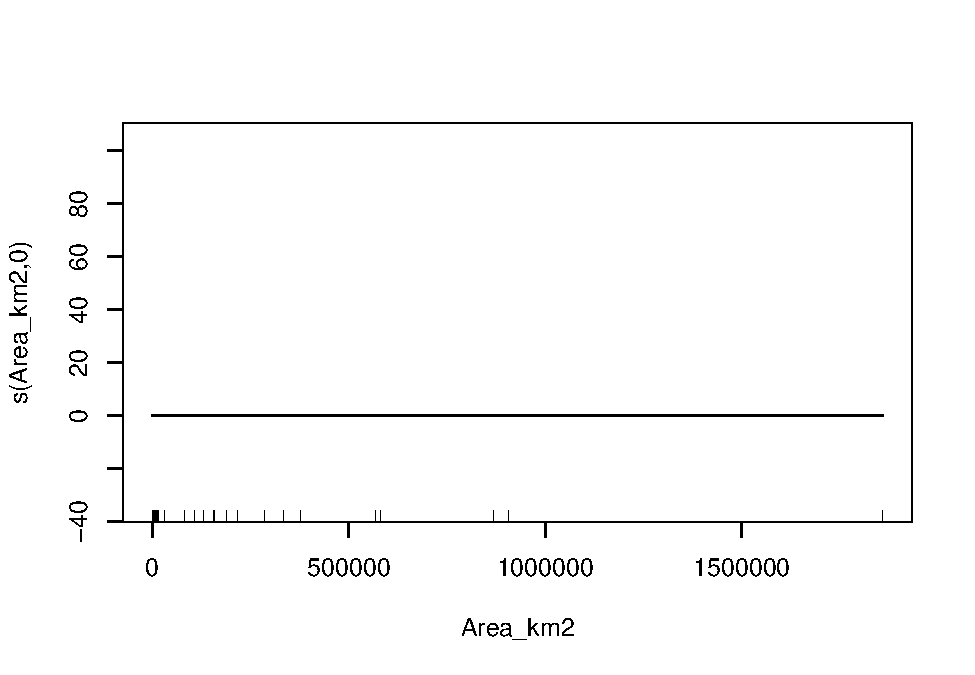
\includegraphics{Forest_and_Water_files/figure-latex/model7_noLatb-2.pdf}

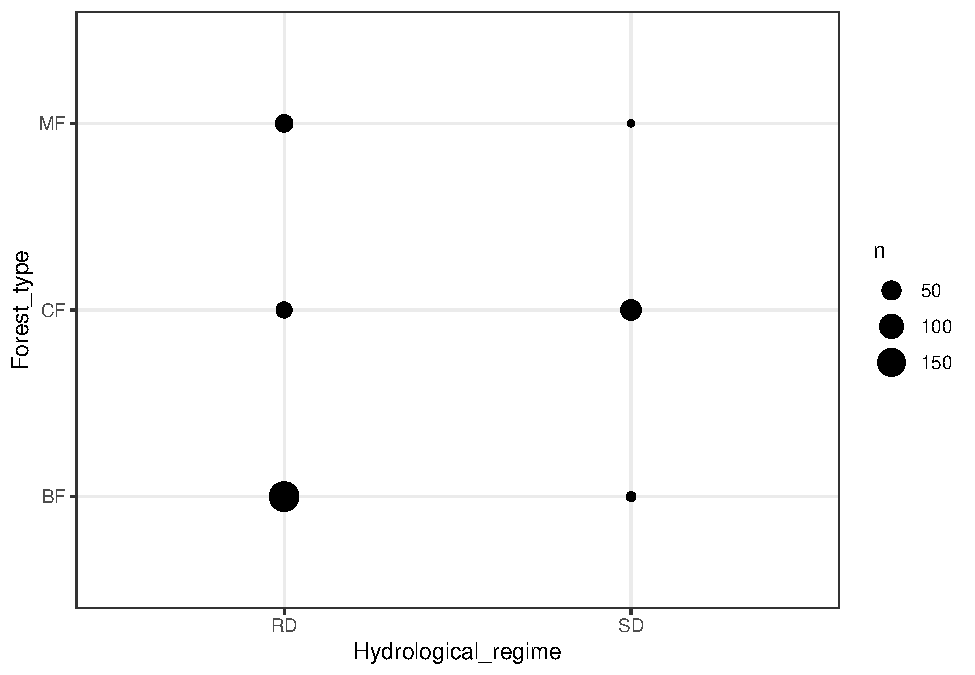
\includegraphics{Forest_and_Water_files/figure-latex/unnamed-chunk-23-1.pdf}

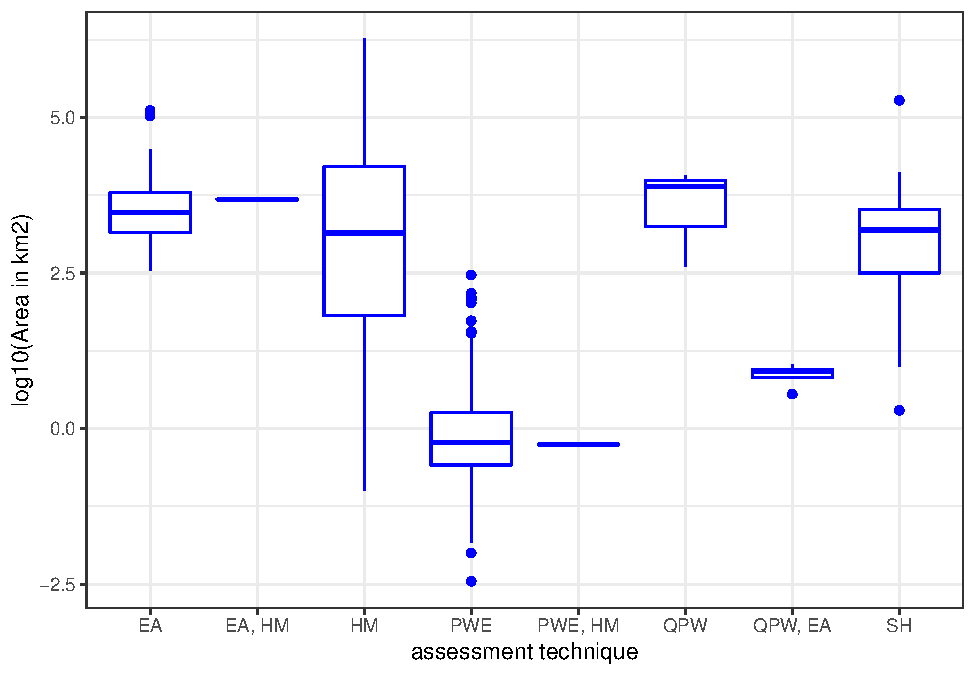
\includegraphics{Forest_and_Water_files/figure-latex/unnamed-chunk-24-1.pdf}

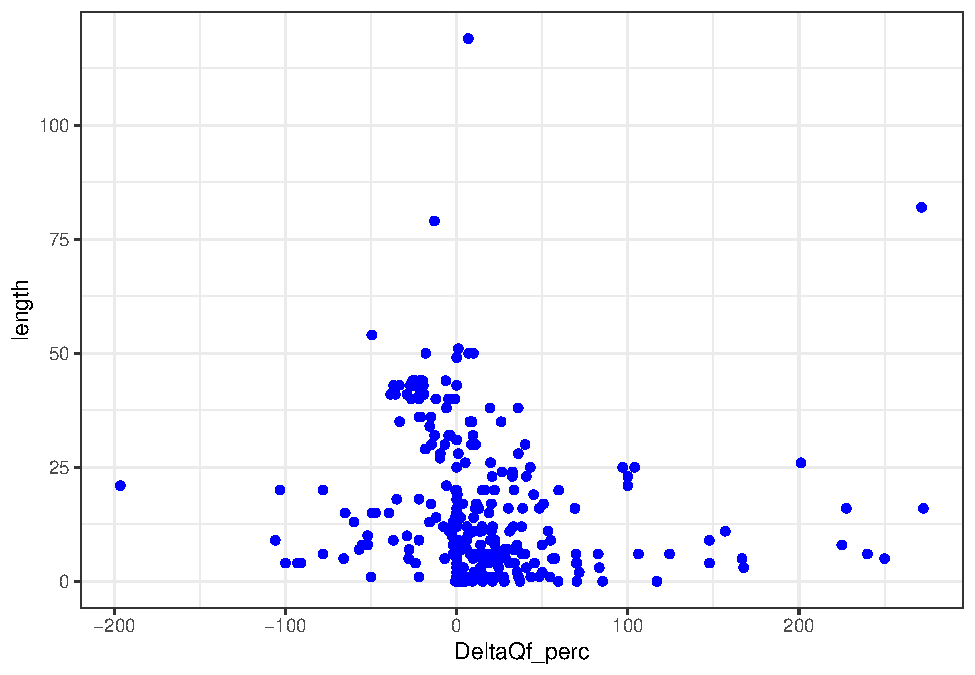
\includegraphics{Forest_and_Water_files/figure-latex/unnamed-chunk-25-1.pdf}

\begin{verbatim}
## pdf 
##   2
\end{verbatim}

\begin{Shaded}
\begin{Highlighting}[]
\NormalTok{Zhang_all2 }\OperatorTok
\StringTok{  }\KeywordTok{ggplot}\NormalTok{(}\KeywordTok{aes}\NormalTok{(Longitude, Latitude, }\DataTypeTok{colour =}\NormalTok{ DeltaF_perc, }\DataTypeTok{size =}\NormalTok{ DeltaQf_perc}\OperatorTok{/}\DecValTok{100}\NormalTok{ )) }\OperatorTok{+}\StringTok{ }\KeywordTok{geom_point}\NormalTok{(}\DataTypeTok{alpha =} \FloatTok{0.5}\NormalTok{)}
\end{Highlighting}
\end{Shaded}

\begin{Shaded}
\begin{Highlighting}[]
\NormalTok{Zhang_all }\OperatorTok
\StringTok{  }\KeywordTok{ggplot}\NormalTok{(}\KeywordTok{aes}\NormalTok{(Area_km2)) }\OperatorTok{+}\StringTok{ }\KeywordTok{geom_histogram}\NormalTok{(}\DataTypeTok{fill=}\StringTok{"blue"}\NormalTok{, }\DataTypeTok{bins =}\DecValTok{50}\NormalTok{) }\OperatorTok{+}
\StringTok{  }\KeywordTok{scale_x_log10}\NormalTok{()}
\NormalTok{total <-}\StringTok{ }\KeywordTok{nrow}\NormalTok{(Zhang_all)}
\KeywordTok{length}\NormalTok{(Zhang_all}\OperatorTok{$}\NormalTok{Area_km2[Zhang_all}\OperatorTok{$}\NormalTok{Area_km2}\OperatorTok{<}\DecValTok{10}\NormalTok{])}\OperatorTok{/}\NormalTok{total}
\end{Highlighting}
\end{Shaded}

\begin{Shaded}
\begin{Highlighting}[]
\NormalTok{Zhang_all2 }\OperatorTok
\StringTok{  }\KeywordTok{ggplot}\NormalTok{(}\KeywordTok{aes}\NormalTok{(length)) }\OperatorTok{+}\StringTok{ }\KeywordTok{geom_histogram}\NormalTok{(}\DataTypeTok{fill=}\StringTok{"blue"}\NormalTok{, }\DataTypeTok{bins =}\DecValTok{50}\NormalTok{) }
\end{Highlighting}
\end{Shaded}

\hypertarget{discussion}{%
\section{Discussion}\label{discussion}}

Essentially, the analysis shows at the moment that in contrast to Zhang
et al. (2017) there is no evidence that the size of a watershed
influences the change in the streamflow as a result of changes in
forestry. If anything the scatter in the data (in the change in flow) is
greater for the smaller watersheds then for the larger watersheds. In
other words, the response to changes in forest cover is more consistent
for larger watersheds than it is for smaller watersheds.

As shown earlier, most of the smaller watersheds are ``real observed
data'' using paired watershed studies, while for larger watersheds, the
analysis are mostly based on modelling approximations using either
elasticity analysis (EA), Hydrological modelling (HM) or a combined use
of statistical methods (SH) or quasi paired watershed analsysi (QPW),
thus all providing an approximation of the effect of forestry on
streamflow rather than a direct comparison of watersheds. This is a
confounding factor that is not easily addressed in the regression
modelling attempted here. Furthermore, the catchments analysed using EA,
are concentrated in the drier end of the Dryness index scale compared to
the other methods, with only the paired watershed experiment (PWE)
assessment technique covering the full range of dryness indices.

There are further confouding factors in the data, which were also
classified by Filoso et al. (2017) and thesse create biases in the data
set that can impact the overall assessment. For example, snow dominated
hydrological regimes (SD), which are weakly significant, are dominated
by Coniferous Forests (CF), while the majority of the rain dominated
regimes are all broadleaf forests (BF). However, the forest type
classification is very coarse and does not fully capture possible
physiological differences that could affect evapotranspiration and
therefore changes in streamflow.

Apart from a difficulty of analysing complex confounding factors in the
data, a general limitation of the type of analysis presented is that
this work does not consider the spatial arrangement of the forest
clearing in the catchments. While for fully or almost fully cleared
smaller catchments this might not be an issue, it is perceivable that
for larger catchments being partially cleared, a interaction between
spatial location and clearing could be a factor in determining the
change in streamflow. Clearing head water catchments on shallower soils
might have a larger impact than clearing in downstream areas on deeper
soils.

\hypertarget{references}{%
\section*{References}\label{references}}
\addcontentsline{toc}{section}{References}

\hypertarget{refs}{}
\leavevmode\hypertarget{ref-andreassian2004}{}%
Andréassian, V., 2004. Waters and forests: From historical controversy
to scientific debate. Journal of Hydrology 291, 1--27.
doi:\href{https://doi.org/https://doi.org/10.1016/j.jhydrol.2003.12.015}{https://doi.org/10.1016/j.jhydrol.2003.12.015}

\leavevmode\hypertarget{ref-borg1988}{}%
Borg, H., Bell, R.W., Loh, I.C., 1988. Streamflow and stream salinity in
a small water supply catchment in southwest western australia after
reforestation. Journal of Hydrology 103, 323--333.
doi:\href{https://doi.org/https://doi.org/10.1016/0022-1694(88)90141-2}{https://doi.org/10.1016/0022-1694(88)90141-2}

\leavevmode\hypertarget{ref-hewlett1984}{}%
Bosch, J.M., Hewlett, J.D., 1982. A review of catchment experiments to
determine the effect of vegetation changes on water yield and
evapotranspiration. Journal of Hydrology 55, 3--23.

\leavevmode\hypertarget{ref-brown2013}{}%
Brown, A.E., Western, A.W., McMahon, T.A., Zhang, L., 2013. Impact of
forest cover changes on annual streamflow and flow duration curves.
Journal of Hydrology 483, 39--50.
doi:\href{https://doi.org/http://dx.doi.org/10.1016/j.jhydrol.2012.12.031}{http://dx.doi.org/10.1016/j.jhydrol.2012.12.031}

\leavevmode\hypertarget{ref-brown2005}{}%
Brown, A.E., Zhang, L., McMahon, T.A., Western, A.W., Vertessy, R.A.,
2005. A review of paired catchment studies for determining changes in
water yield resulting from alterations in vegetation. Journal of
Hydrology 310, 28--61.

\leavevmode\hypertarget{ref-cosandey2005}{}%
Cosandey, C., Andréassian, V., Martin, C., Didon-Lescot, J.F., Lavabre,
J., Folton, N., Mathys, N., Richard, D., 2005. The hydrological impact
of the mediterranean forest: A review of french research. Journal of
Hydrology 301, 235--249.
doi:\href{https://doi.org/https://doi.org/10.1016/j.jhydrol.2004.06.040}{https://doi.org/10.1016/j.jhydrol.2004.06.040}

\leavevmode\hypertarget{ref-filoso2017}{}%
Filoso, S., Bezerra, M.O., Weiss, K.C.B., Palmer, M.A., 2017. Impacts of
forest restoration on water yield: A systematic review. PLOS ONE 12,
e0183210.
doi:\href{https://doi.org/10.1371/journal.pone.0183210}{10.1371/journal.pone.0183210}

\leavevmode\hypertarget{ref-jackson2005}{}%
Jackson, R.B., Jobbagy, E.G., Avissar, R., Roy, S.B., Barrett, D.J.,
Cook, C.W., Farley, K.A., Maitre, D.C. le, McCarl, B.A., Murray, B.C.,
2005. Trading water for carbon with biological carbon sequestration.
Science 310, 1944--1947.
doi:\href{https://doi.org/10.1126/science.1119282}{10.1126/science.1119282}

\leavevmode\hypertarget{ref-pena-arancibia2012}{}%
Peña-Arancibia, J.L., Dijk, A.I.J.M. van, Guerschman, J.P., Mulligan,
M., Bruijnzeel, L.A., McVicar, T.R., 2012. Detecting changes in
streamflow after partial woodland clearing in two large catchments in
the seasonal tropics. Journal of Hydrology 416-417, 60--71.
doi:\href{https://doi.org/https://doi.org/10.1016/j.jhydrol.2011.11.036}{https://doi.org/10.1016/j.jhydrol.2011.11.036}

\leavevmode\hypertarget{ref-roche1981}{}%
Roche, M., 1981. Watershed investigations for development of forest
resources of the amazon region in french guyana. Tropical Agricultural
Hydrology. J 75--82.

\leavevmode\hypertarget{ref-rodriguez2010}{}%
Rodriguez, D.A., Tomasella, J., Linhares, C., 2010. Is the forest
conversion to pasture affecting the hydrological response of amazonian
catchments? Signals in the ji-paraná basin. Hydrological Processes 24,
1254--1269.
doi:\href{https://doi.org/https://doi.org/10.1002/hyp.7586}{https://doi.org/10.1002/hyp.7586}

\leavevmode\hypertarget{ref-ruprechtetal1991}{}%
Ruprecht, J.K., Schofield, N.J., Crombie, D.S., Vertessy, R.A.,
Stoneman, G.L., 1991. Early hydrological response to intense forest
thinning in southwestern australia. Journal of Hydrology 127, 261--277.
doi:\href{https://doi.org/https://doi.org/10.1016/0022-1694(91)90118-2}{https://doi.org/10.1016/0022-1694(91)90118-2}

\leavevmode\hypertarget{ref-thornton2007}{}%
Thornton, C.M., Cowie, B.A., Freebairn, D.M., Playford, C.L., 2007. The
brigalow catchment study: II*. Clearing brigalow (acacia harpophylla)
for cropping or pasture increases runoff. Australian Journal of Soil
Research 45, 496--511.
doi:\href{https://doi.org/doi:10.1071/SR07064}{doi:10.1071/SR07064}

\leavevmode\hypertarget{ref-trabucco2018}{}%
Trabucco, A., Zomer, R.J., 2018. Global aridity index and potential
evapo-transpiration (et0) climate database v2. CGIAR consortium for
spatial information(CGIAR-csi).

\leavevmode\hypertarget{ref-wood2006}{}%
Wood, S., 2006. Generalized additive models: An introduction with r. CRC
Press, Boca Raton, FL.

\leavevmode\hypertarget{ref-zhang2011}{}%
Zhang, L., Zhao, F., Chen, Y., Dixon, R.N.M., 2011. Estimating effects
of plantation expansion and climate variability on streamflow for
catchments in australia. Water Resources Research 47, W12539.
doi:\href{https://doi.org/10.1029/2011wr010711}{10.1029/2011wr010711}

\leavevmode\hypertarget{ref-zhang2017}{}%
Zhang, M., Liu, N., Harper, R., Li, Q., Liu, K., Wei, X., Ning, D., Hou,
Y., Liu, S., 2017. A global review on hydrological responses to forest
change across multiple spatial scales: Importance of scale, climate,
forest type and hydrological regime. Journal of Hydrology 546, 44--59.
doi:\href{https://doi.org/https://doi.org/10.1016/j.jhydrol.2016.12.040}{https://doi.org/10.1016/j.jhydrol.2016.12.040}

\leavevmode\hypertarget{ref-zhao2010}{}%
Zhao, F., Zhang, L., Xu, Z., Scott, D.F., 2010. Evaluation of methods
for estimating the effects of vegetation change and climate variability
on streamflow. Water Resources Research 46, W03505.
doi:\href{https://doi.org/10.1029/2009wr007702}{10.1029/2009wr007702}

\leavevmode\hypertarget{ref-zhou2015}{}%
Zhou, G., Wei, X., Chen, X., Zhou, P., Liu, X., Xiao, Y., Sun, G.,
Scott, D.F., Zhou, S., Han, L., Su, Y., 2015. Global pattern for the
effect of climate and land cover on water yield. Nature Communications
6, 5918.
doi:\href{https://doi.org/10.1038/ncomms6918}{10.1038/ncomms6918}

\leavevmode\hypertarget{ref-zhou2010}{}%
Zhou, G., Wei, X., Luo, Y., Zhang, M., Li, Y., Qiao, Y., Liu, H., Wang,
C., 2010. Forest recovery and river discharge at the regional scale of
guangdong province, china. Water Resources Research 46.
doi:\href{https://doi.org/https://doi.org/10.1029/2009WR008829}{https://doi.org/10.1029/2009WR008829}


\end{document}


